\documentclass[a4paper]{article}

\usepackage[utf8]{inputenc}
\usepackage{geometry}
\geometry{left=2.5cm, right=2.5cm, top=2cm, bottom=2cm}
\usepackage{microtype}
\usepackage{graphicx}
\usepackage{amsmath, amssymb, amsthm}
\usepackage{float}
\usepackage{hyperref}
\usepackage{caption}
\usepackage{subcaption}
\usepackage{listings}
\usepackage[table]{xcolor}
\usepackage{fancyhdr}
\usepackage{lastpage}
\usepackage{booktabs}
\captionsetup[table]{skip=4pt}
\linespread{1.1}

\pagestyle{fancy}
\fancyhead[R]{\hmwkAuthorName}
\fancyhead[L]{\hmwkClass: \hmwkTitle}
\fancyfoot[L]{}   % Bottom left footer
\fancyfoot[C]{}   % Bottom center footer
\fancyfoot[R]{Page\ \thepage\ of\ \pageref{LastPage}} % Bottom right footer

\renewcommand\headrulewidth{0.4pt}
\renewcommand\footrulewidth{0.4pt}

\definecolor{MyDarkGreen}{rgb}{0.0,0.4,0.0}
\definecolor{shadecolor}{gray}{0.9}
\definecolor{codegreen}{rgb}{0,0.6,0}
\definecolor{codegray}{rgb}{0.5,0.5,0.5}
\definecolor{codepurple}{rgb}{0.58,0,0.82}
\definecolor{backcolour}{rgb}{0.96,0.96,0.94}

% Style configuration
\lstdefinestyle{mystyle}{
    backgroundcolor=\color{backcolour},   
    commentstyle=\color{codegreen},
    keywordstyle=\color{magenta},
    numberstyle=\tiny\color{codegray},
    stringstyle=\color{codepurple},
    basicstyle=\ttfamily\footnotesize,
    breakatwhitespace=false,         
    breaklines=true,                 
    captionpos=b,                    
    keepspaces=true,                 
    numbers=left,                    
    numbersep=5pt,                  
    showspaces=false,                
    showstringspaces=false,
    showtabs=false,                  
    tabsize=4,
    language=Python
}

\lstset{style=mystyle}

\newcommand{\hmwkTitle}{Assignment 1}
\newcommand{\hmwkClass}{INT 3404 – Image Processing}
\newcommand{\hmwkAuthorName}{Dang Dinh Khang - 23020675}

\title{
    \textbf{INT 3404: IMAGE PROCESSING} \\
    \vspace{0.5cm}
    \Large \textbf{Assignment 1: The Digital Camera Pipeline}
}
\author{
    \textbf{Student Name: } Dang Dinh Khang \\
    \textbf{Student ID: } 23020675
}
\date{October 15, 2026}

\begin{document}

\maketitle

\section{Introduction}
\label{Introduction}

Digital camera sensors capture physical scene radiance by accumulating photons on an array of photodiodes overlaid with a Color Filter Array (CFA). These raw measurements do not form a directly viewable image: they are recorded in a camera-specific, device-dependent coordinate system, contain substantial dark current offsets, exhibit a sparse single-color-per-pixel mosaic, and behave strictly linearly with respect to incident photon flux.

In this assignment, I implement the complete \textbf{Digital Camera Pipeline} (Image Signal Processor - ISP) from scratch in Python to transform the raw sensor data of \texttt{campus.CR2} (captured with a Canon EOS 5D Mark III DSLR) into an accurate, aesthetically pleasing, and standardized sRGB image. The sequential pipeline includes:
\begin{enumerate}
    \item \textbf{Raw Image Extraction}: Extracting metadata and pure linear sensor measurements using \texttt{dcraw}.
    \item \textbf{Linearization}: Normalizing pixel values by eliminating dark current offsets and mapping to $[0, 1]$.
    \item \textbf{Bayer Mosaic Masking \& Phase Identification}: Establishing color channel masks and determining the correct Bayer phase.
    \item \textbf{White Balancing}: Correcting illuminant color casts via four standard algorithms.
    \item \textbf{Demosaicing}: Reconstructing a dense three-channel RGB representation using 2D bilinear convolution kernels.
    \item \textbf{Color Space Correction}: Transforming device-dependent camera RGB coordinates to standard sRGB via CIE XYZ 1931 space.
    \item \textbf{Brightness Scaling \& Gamma Encoding}: Adjusting exposure to target perceptual middle gray and applying non-linear sRGB gamma encoding.
    \item \textbf{Image Compression}: Evaluating lossless PNG versus lossy JPEG compression across quality factors.
\end{enumerate}

\section{Raw Image Extraction}

\subsection{Reconnaissance}
Before performing any image operations, I inspected the sensor-specific metadata using the command-line utility \texttt{dcraw}~\cite{dcraw}:
\begin{lstlisting}[language=bash, numbers=none]
dcraw -4 -d -v -w -T campus.CR2
\end{lstlisting}
The output produced by \texttt{dcraw} is:
\begin{lstlisting}[language=bash, numbers=none]
Loading Canon EOS 5D Mark III image from campus.CR2 ...
Scaling with darkness 2048, saturation 15488, and multipliers 1.858398 1.000000 1.723633 1.000000
\end{lstlisting}
From this output, the critical calibration parameters are identified:
\begin{itemize}
    \item \textbf{Camera Model:} Canon EOS 5D Mark III
    \item \textbf{Darkness (Black Level):} $2048$
    \item \textbf{Saturation (White Level):} $15488$
    \item \textbf{White Balance Multipliers ($r_{\text{scale}}, g_{\text{scale}}, b_{\text{scale}}, g_{\text{scale}}$):} $[1.858398, 1.000000, 1.723633, 1.000000]$
\end{itemize}

\subsection{Generating the Linear TIFF}
\label{load_raw_tiff}
Using \texttt{dcraw -4 -D -T campus.CR2}, I generated a linear 16-bit TIFF file, preserving the completely unscaled, un-interpolated raw sensor data. This TIFF file serves as the input for the subsequent steps in the camera pipeline. My implementation of the \texttt{load\_raw\_tiff} function is as follows:

\begin{lstlisting}
def load_raw_tiff(self):
    raw = io.imread(self.tiff_path)
    self.raw_image = raw.astype(np.float64)

    h, w = self.raw_image.shape[:2]
    min_val = self.raw_image.min()
    max_val = self.raw_image.max()
    approx_bpp = np.log2(max_val + 1)

    print(f"Image Width: {w}, Image Height: {h}")
    print(f"Min raw value: {min_val}, Max raw value: {max_val}")
    print(f"Approximate bits per pixel: {approx_bpp:.2f} (container: {raw.dtype})")
    return self.raw_image
\end{lstlisting}

The resulting \textbf{raw\_image} attributes are:
\begin{itemize}
    \item \textbf{Image Dimensions:} $5796 \times 3870$ (Width $\times$ Height)
    \item \textbf{Min Raw Value:} $2029.0$
    \item \textbf{Max Raw Value:} $16383.0$
    \item \textbf{Bit Depth:} $14$ bits per pixel, since $\log_2(16383 + 1) = 14.00$. The TIFF file merely stores these 14-bit sensor values inside 16-bit words (\texttt{uint16}); the two most significant bits are never used.
\end{itemize}

\section{Linearization}
Silicon photodiodes generate thermal electrons even in complete darkness, producing a non-zero signal offset known as \textit{Dark Current}. Conversely, when photodiode electron wells reach full capacity, saturation occurs. To ensure recorded digital numbers accurately correspond to physical scene radiance, the raw readings $P_{\text{raw}}$ must be linearized and normalized onto $[0.0, 1.0]$:
\begin{equation}
    P_{\text{linear}} = \text{clip}\left(\frac{P_{\text{raw}} - \text{black}}{\text{white} - \text{black}}, 0.0, 1.0\right)
\end{equation}
where $\text{black} = 2048$ and $\text{white} = 15488$. Values $\le 2048$ represent absolute black ($0.0$), values $\ge 15488$ represent sensor saturation ($1.0$), and intermediate intensities scale linearly.

\begin{lstlisting}
def linearize(self):
    if self.raw_image is None:
        raise ValueError("Raw image is not loaded.")
    p_linear = (self.raw_image - self.black) / (self.white - self.black)
    self.linear_image = np.clip(p_linear, 0.0, 1.0)
    return self.linear_image
\end{lstlisting}

\section{The Bayer Pattern}

\subsection{The Bayer Pattern Design}
The Bayer Color Filter Array (CFA)~\cite{bayer1976} arranges red, green, and blue color filters in a repeating $2 \times 2$ tessellation with $50\%$ Green, $25\%$ Red, and $25\%$ Blue pixels. The physical and biological rationale is designed to mimic the Spectral Sensitivity Function of the human eye:

\begin{itemize}
    \item \textbf{Human Perception:} The eye's peak sensitivity lies in the green spectrum ($\sim 555\text{ nm}$), with Medium (M) and Long (L) cone cells making humans far more receptive to green light.
    \item \textbf{Luminance \& Detail:} The human visual system (HVS) derives most luminance (brightness) and fine spatial detail from green wavelengths, while Red and Blue primarily contribute to chrominance (color).
    \item \textbf{Sensor Allocation:} In a $2 \times 2$ Bayer pattern, allocating 2 cells to Green ($50\%$) and 1 cell each to Red and Blue ($25\%$) maximizes perceived sharpness and dynamic range where human vision is most sensitive.
\end{itemize}

The function \texttt{\_build\_bayer\_masks} constructs the boolean masks of the three channels for any of the four phases:
\begin{lstlisting}
@staticmethod
def _build_bayer_masks(h, w, pattern):
    pattern = pattern.upper()
    mask_r = np.zeros((h, w), dtype=bool)
    mask_g = np.zeros((h, w), dtype=bool)
    mask_b = np.zeros((h, w), dtype=bool)
    channel_masks = {'R': mask_r, 'G': mask_g, 'B': mask_b}
    tile_positions = [
        (slice(0, h, 2), slice(0, w, 2)),
        (slice(0, h, 2), slice(1, w, 2)),
        (slice(1, h, 2), slice(0, w, 2)),
        (slice(1, h, 2), slice(1, w, 2)),
    ]
    for char, (row_slice, col_slice) in zip(pattern, tile_positions):
        if char in channel_masks:
            channel_masks[char][row_slice, col_slice] = True
    return mask_r, mask_g, mask_b
\end{lstlisting}

\subsection{Identifying the Correct Pattern Phase}
\label{sec:phase}
Because the $2 \times 2$ filter repeats across the sensor, the color of the coordinate $(0, 0)$ determines one of four possible pattern phases: \texttt{RGGB}, \texttt{BGGR}, \texttt{GRBG}, or \texttt{GBRG}. I used two independent strategies, and both give \textbf{\texttt{RGGB}}.

\paragraph{How intermediate images are displayed.} Every image shown in Sections 4--7 is rendered without the brightness scaling and gamma encoding of Section 8: the linear values in $[0, 1]$ are written directly as 8-bit pixels ($\times 255$). The images therefore look dark at this point of the pipeline; Section 8 explains why. Each caption states the step after which the image was taken.

\subsubsection{Strategy 1: Visual comparison after demosaicing}
Each of the four pattern strings is passed to the pipeline, which is run only as far as demosaicing: linearization $\rightarrow$ white balancing (camera presets, as advised in the assignment) $\rightarrow$ bilinear demosaicing. No color space correction or brightness adjustment is applied. Figure~\ref{fig:pattern_comparison} shows the four interpolated images.

\begin{figure}[H]
    \centering
    \begin{subfigure}[b]{0.48\textwidth}
        \centering
        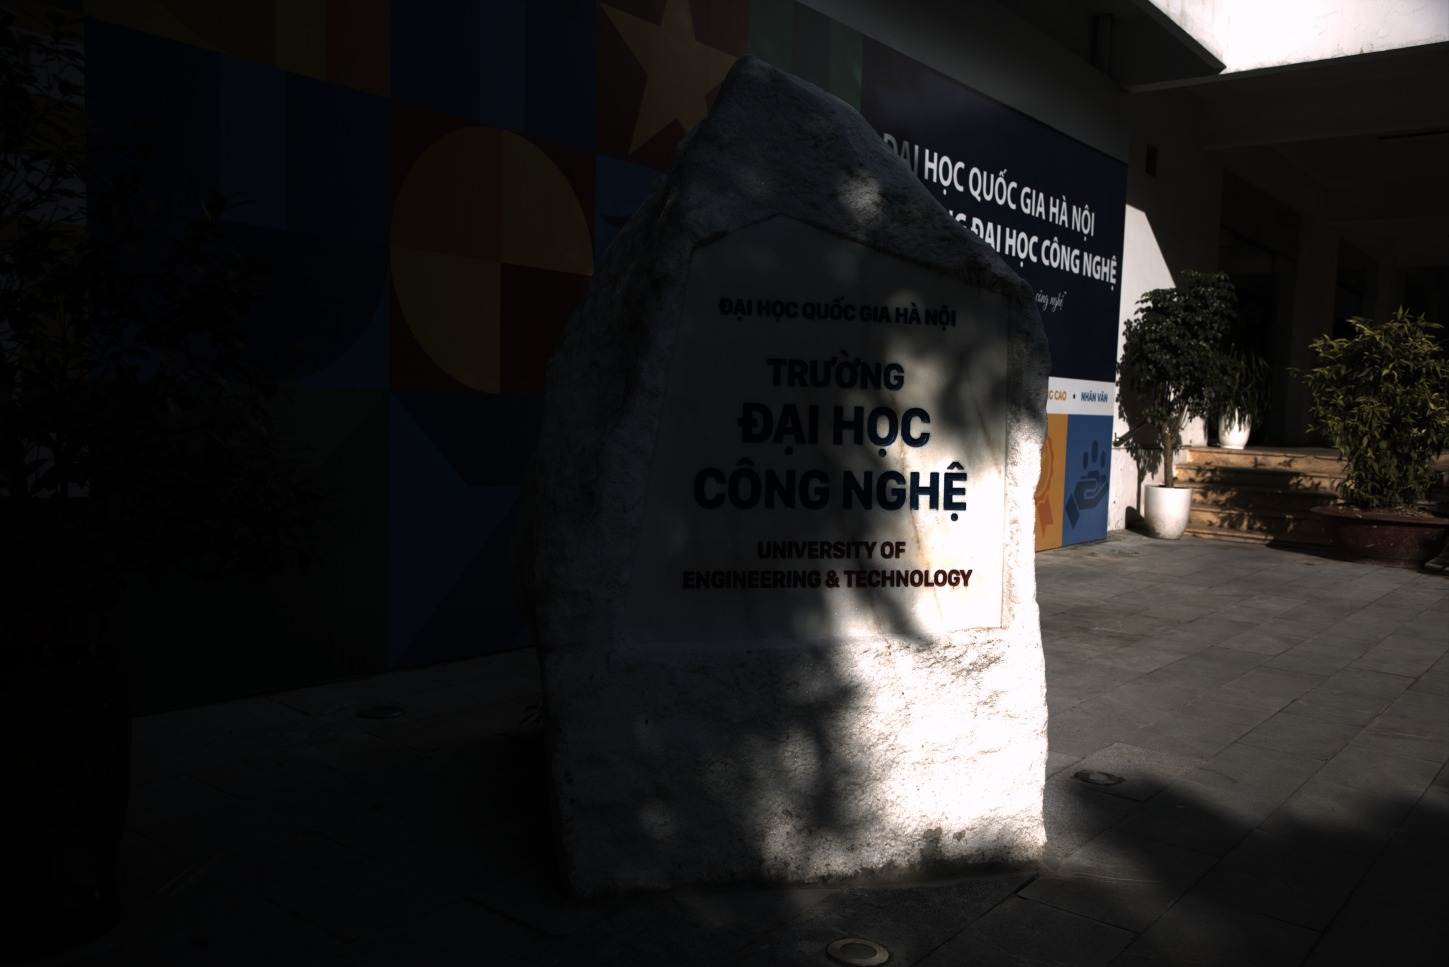
\includegraphics[width=\textwidth]{figures/pattern_rggb.jpg}
        \caption{\texttt{RGGB} (correct phase)}
        \label{fig:pat_rggb}
    \end{subfigure}
    \hfill
    \begin{subfigure}[b]{0.48\textwidth}
        \centering
        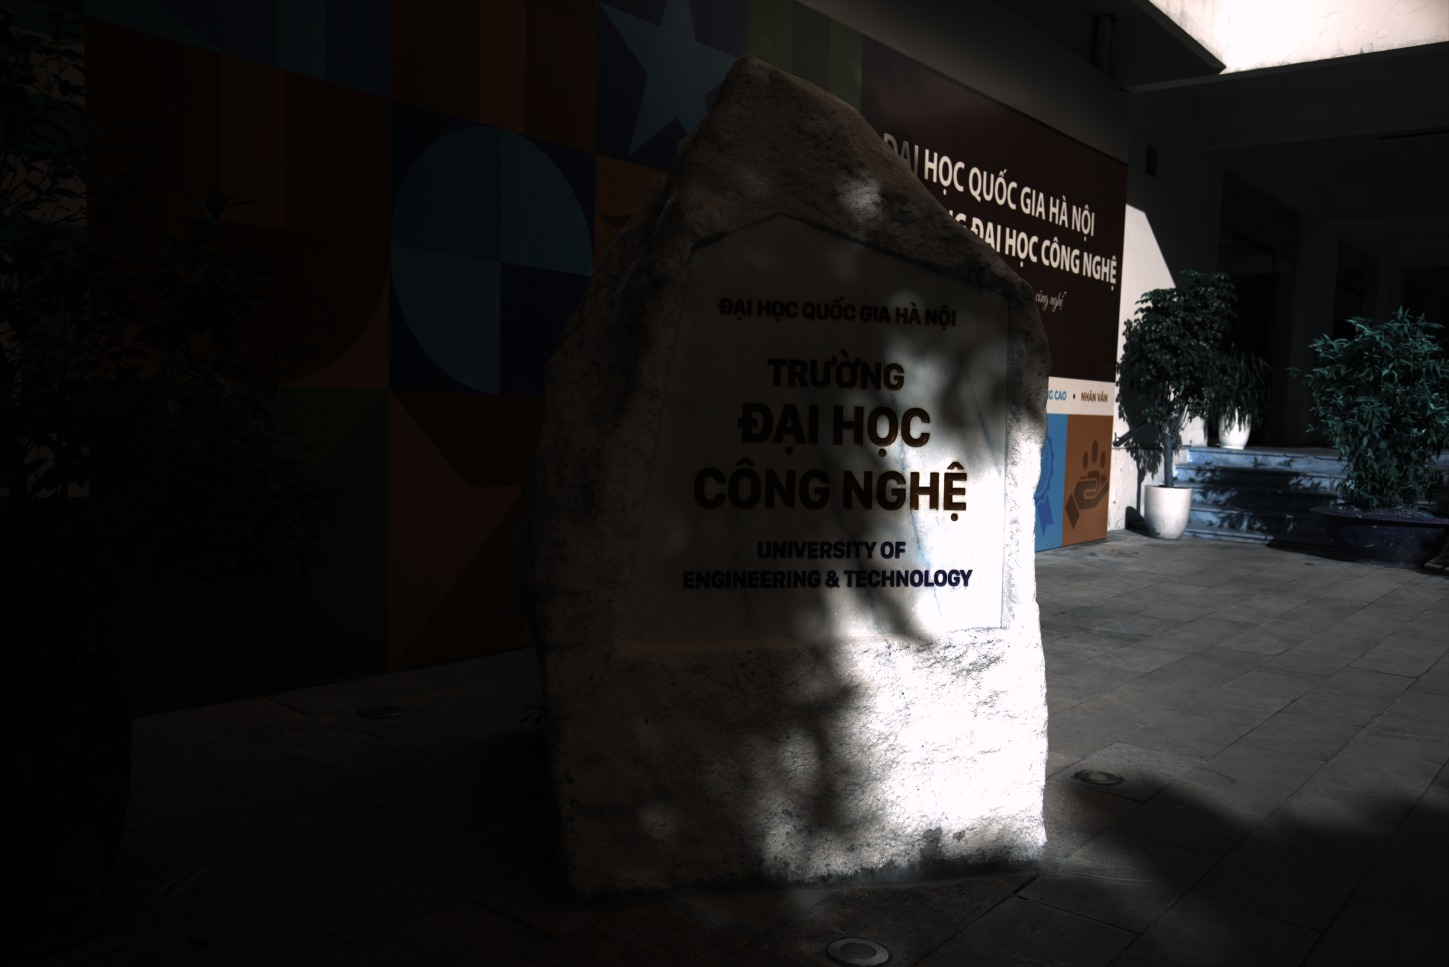
\includegraphics[width=\textwidth]{figures/pattern_bggr.jpg}
        \caption{\texttt{BGGR} (red and blue swapped)}
        \label{fig:pat_bggr}
    \end{subfigure}

    \vspace{0.3cm}
    \begin{subfigure}[b]{0.48\textwidth}
        \centering
        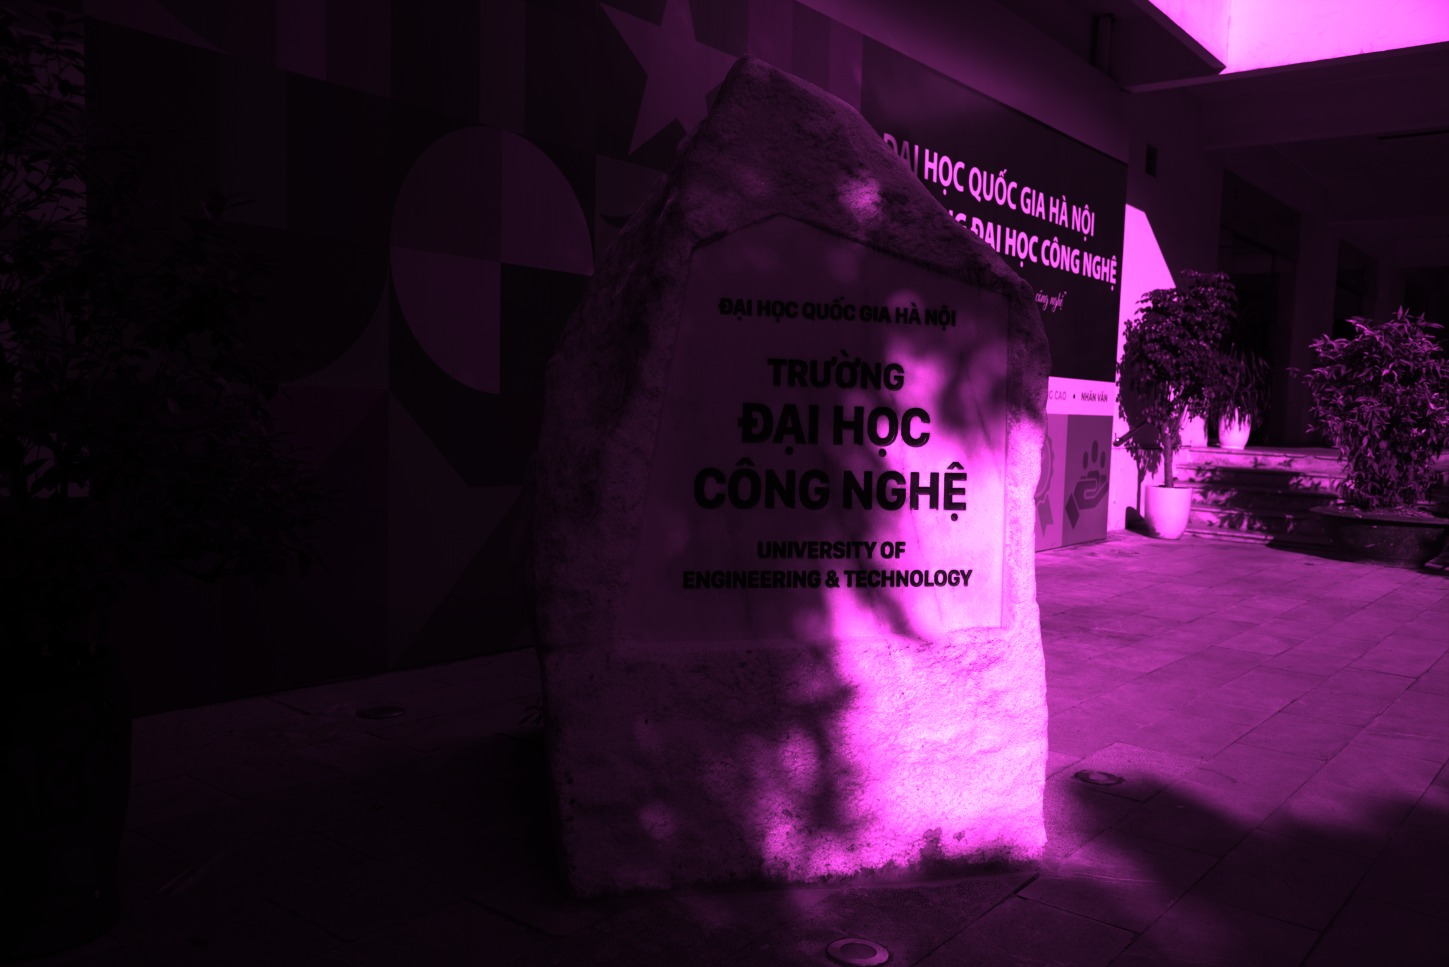
\includegraphics[width=\textwidth]{figures/pattern_grbg.jpg}
        \caption{\texttt{GRBG} (shifted by one column)}
        \label{fig:pat_grbg}
    \end{subfigure}
    \hfill
    \begin{subfigure}[b]{0.48\textwidth}
        \centering
        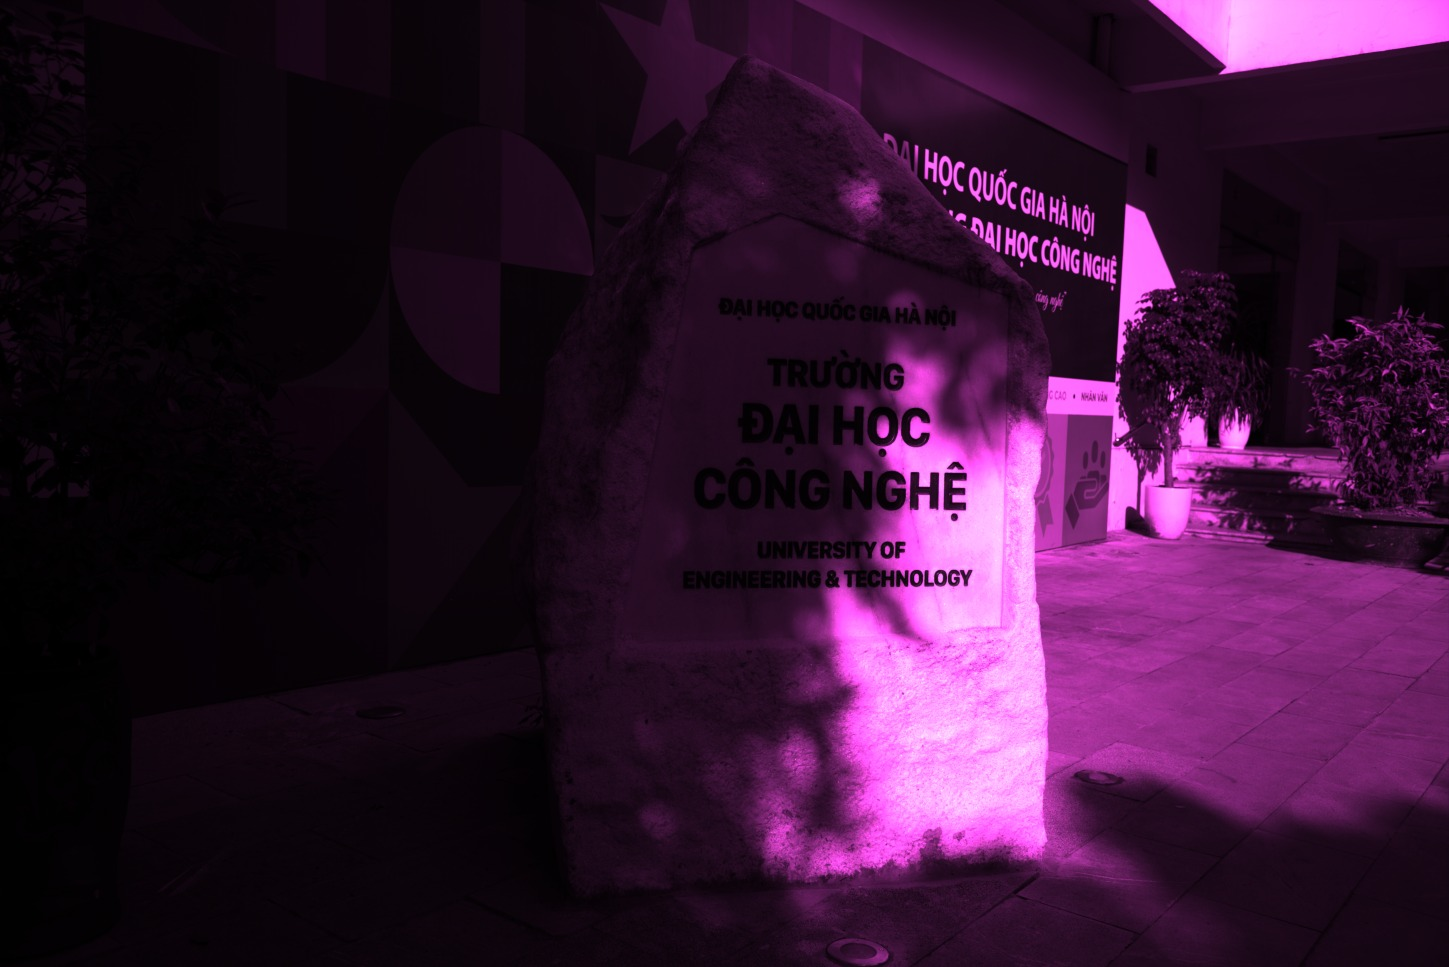
\includegraphics[width=\textwidth]{figures/pattern_gbrg.jpg}
        \caption{\texttt{GBRG} (shifted by one row)}
        \label{fig:pat_gbrg}
    \end{subfigure}
    \caption{The four Bayer phases, each shown directly after the demosaicing step (white-balanced with the camera presets, no color correction).}
    \label{fig:pattern_comparison}
\end{figure}

\begin{itemize}
    \item \textbf{\texttt{RGGB}:} the white stone is neutral, the potted plants are green, and the blue, orange and yellow panels of the mural can be made out. The image is dark because it is still linear, and the colors are muted because it is still in camera RGB, but they are plausible.
    \item \textbf{\texttt{BGGR}:} green stays in place, but red and blue are exchanged. The orange panels of the mural become blue and the blue panels become brown/orange, the red inscription turns blue, and the white stone takes a beige tint because the red and blue gains are applied to the wrong channels.
    \item \textbf{\texttt{GRBG} and \texttt{GBRG}:} the pixels treated as ``green'' are actually the sensor's red and blue pixels, while the true green samples are sent to the red and blue channels and amplified by the white balance gains. The whole image turns magenta, including the plants, which is impossible for this scene.
\end{itemize}

\subsubsection{Strategy 2: Reading the pattern from the bytes of the RAW file}
\label{sec:cr2_bytes}
A RAW decoder has to know the Bayer phase before it can demosaic, and it obtains it from the RAW file. I implemented this process as a pipeline method, \texttt{detect\_bayer\_pattern\_from\_cr2()}, which reads \texttt{campus.CR2} byte by byte in plain Python, without any imaging or metadata library, and stores the pattern it finds in the pipeline before demosaicing.

\paragraph{Structure of a CR2 file.} CR2 (Canon RAW version 2) is built on the TIFF format~\cite{lclevy_cr2, libopenraw_cr2}. Figure~\ref{fig:cr2_poster} shows its layout: a TIFF header and a CR2 header, then a chain of four \emph{Image File Directories} (IFD\#0 to IFD\#3) with the EXIF and Canon MakerNote sub-IFDs attached to IFD\#0, and finally the image data. IFD\#0 to IFD\#2 describe preview images, while IFD\#3 describes the RAW sensor data. Every IFD has the same structure:
\begin{itemize}
    \item 2 bytes: the number of entries $n$;
    \item $n$ entries of 12 bytes each: tag (2 bytes), data type (2 bytes), count (4 bytes), and the value itself or, if it does not fit in 4 bytes, the offset where it is stored (4 bytes);
    \item 4 bytes: the offset of the next IFD ($0$ for the last one).
\end{itemize}
All offsets are counted in bytes from the beginning of the file.

\begin{figure}[H]
    \centering
    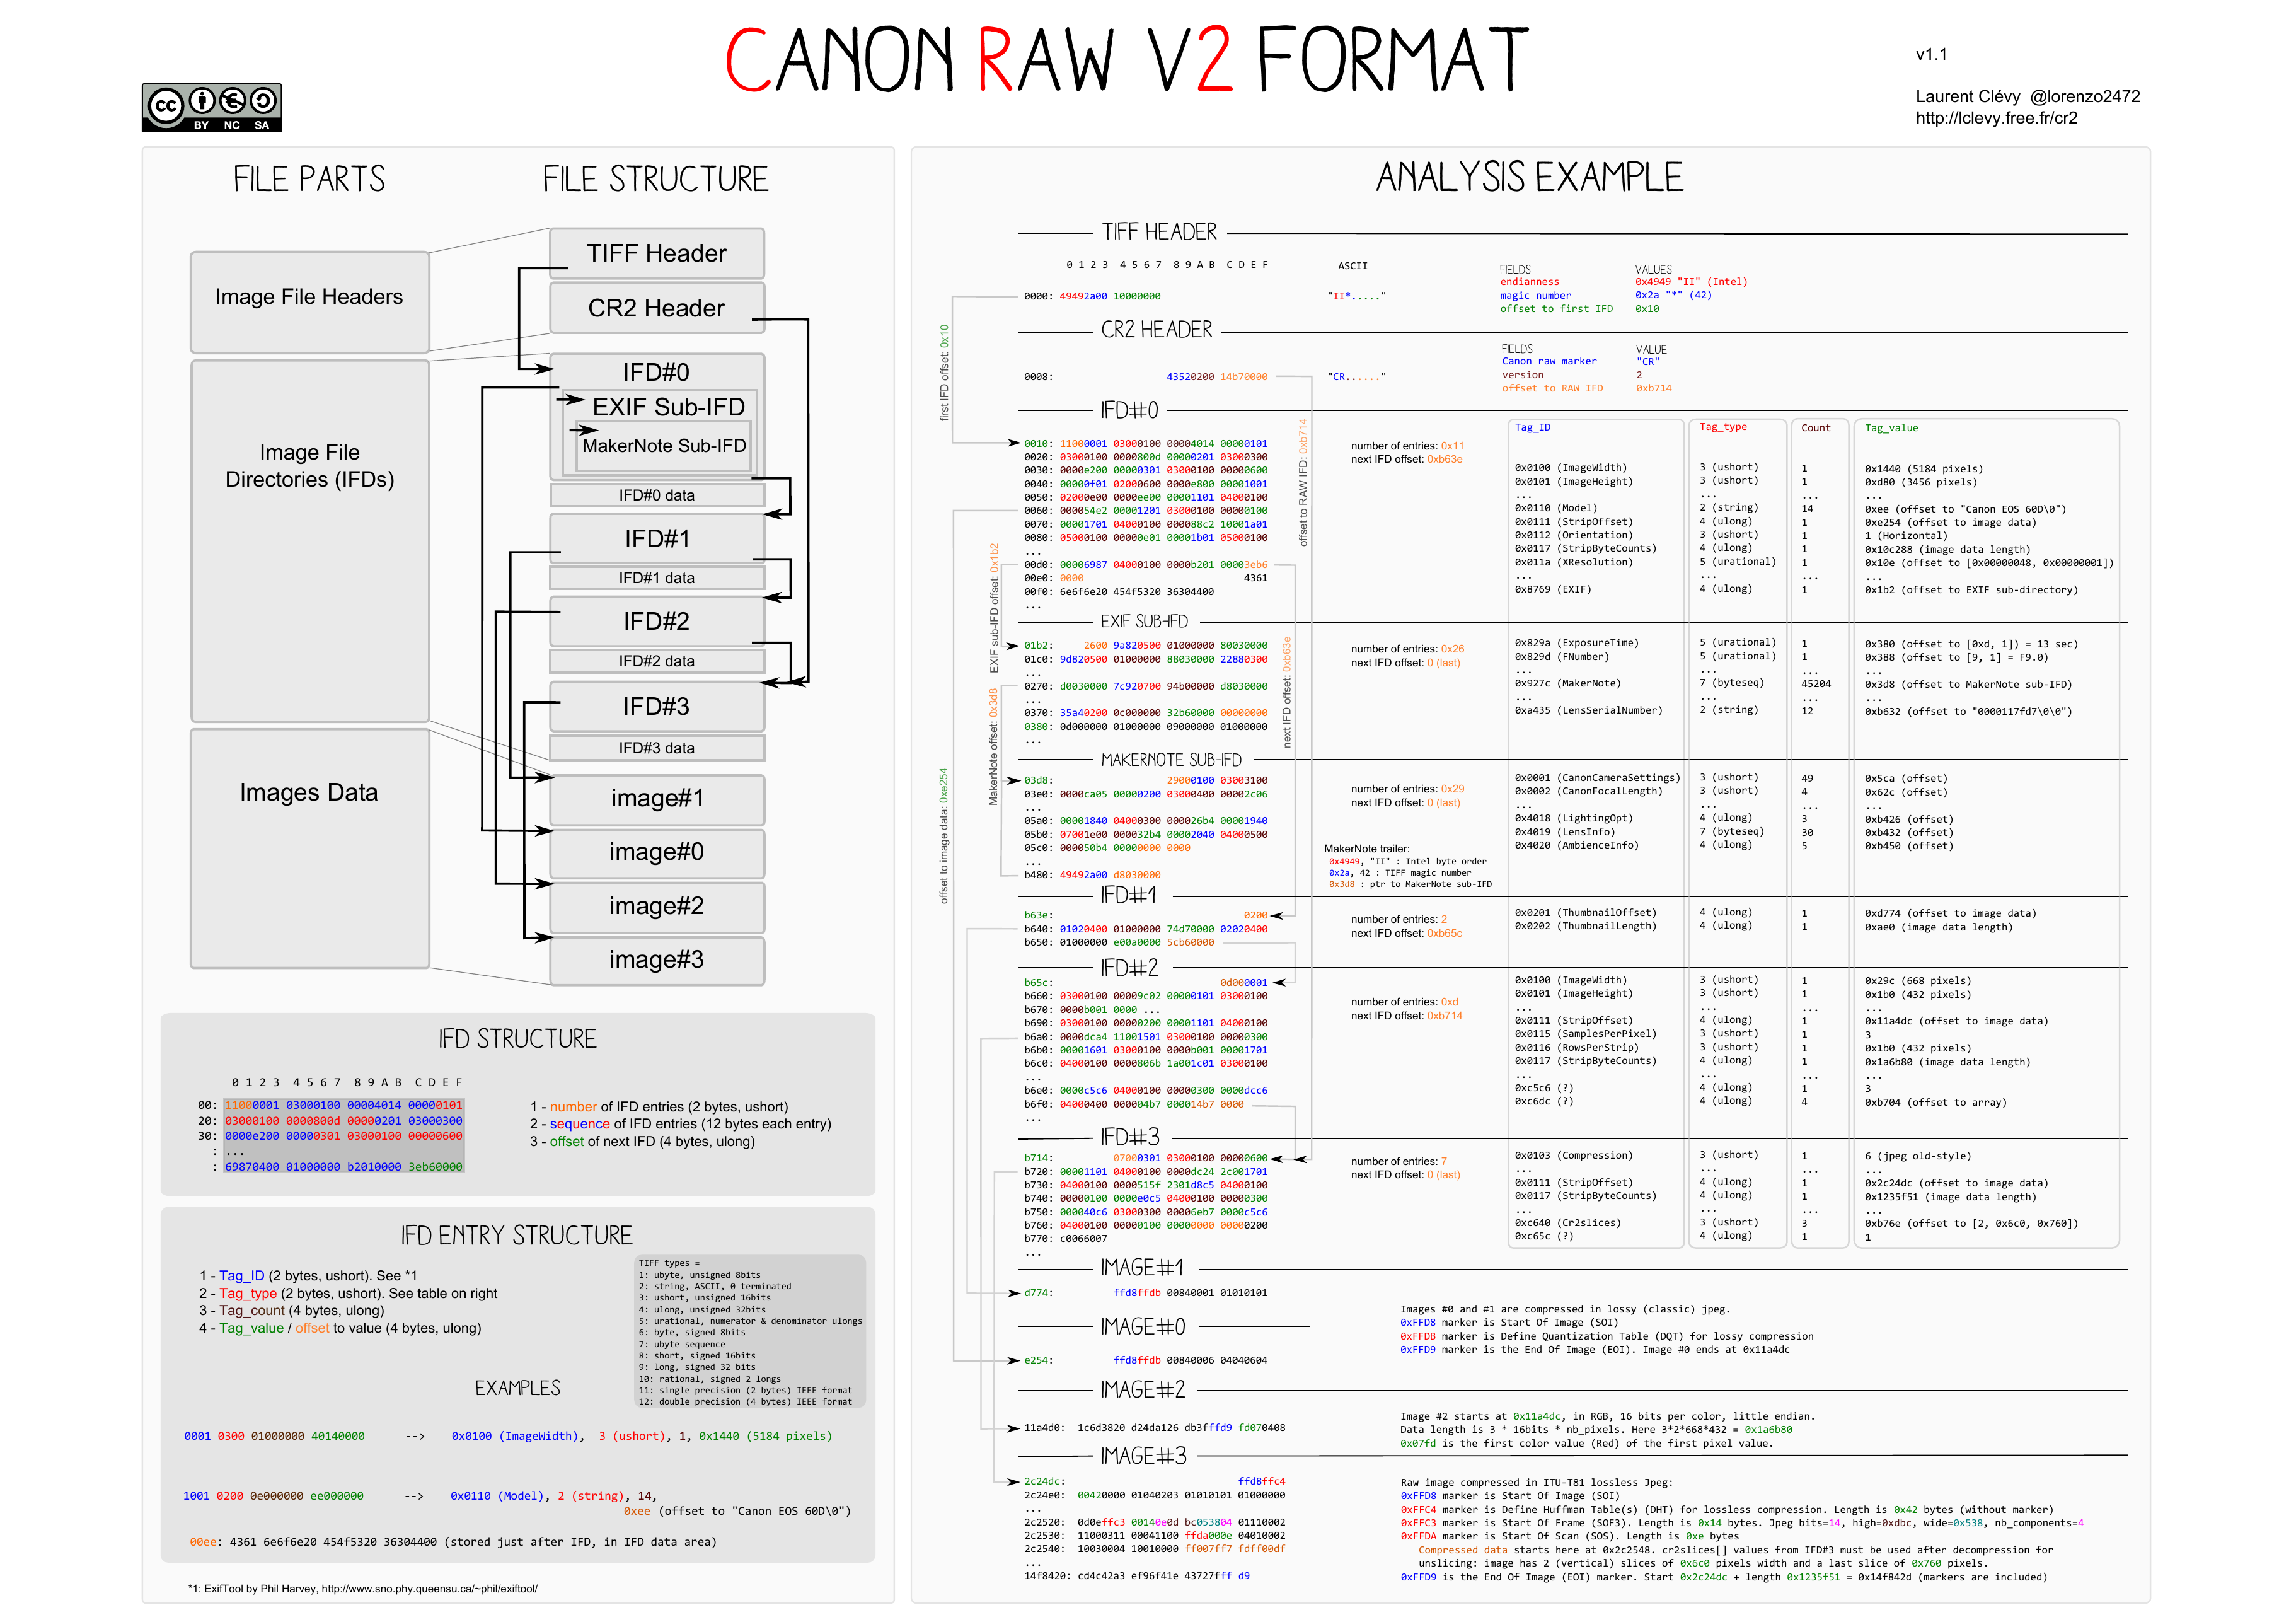
\includegraphics[width=\textwidth]{figures/cr2_format_poster.png}
    \caption{Structure of a CR2 file (left) and an annotated analysis of an example file (right). Poster ``Canon Raw v2 Format'' v1.1 by Laurent Cl\'{e}vy~\cite{lclevy_poster}, licensed under CC BY-NC-SA 4.0.}
    \label{fig:cr2_poster}
\end{figure}

The bytes quoted below are those of \texttt{campus.CR2}, displayed with \texttt{hexdump -C -s <offset> -n <length> campus.CR2}. Only the parts of the file that are needed to find the Bayer pattern are read.

\paragraph{Step 1: TIFF and CR2 headers.} The first 16 bytes of the file are
\begin{lstlisting}[language={}, numbers=none]
00000000  49 49 2a 00 10 00 00 00  43 52 02 00 80 19 01 00  |II*.....CR......|
\end{lstlisting}
\begin{itemize}
    \item Bytes 0--1, \texttt{49 49} (``II''): the file is \emph{little-endian} (Intel order), so every multi-byte number is read from its last byte to its first.
    \item Bytes 2--3, \texttt{2a 00} $\rightarrow$ \texttt{0x002A} $= 42$: the TIFF identifier.
    \item Bytes 4--7, \texttt{10 00 00 00} $\rightarrow$ \texttt{0x10}: offset of IFD\#0.
    \item Bytes 8--11, \texttt{43 52 02 00}: the CR2 marker ``CR'' and version $2.0$.
    \item Bytes 12--15, \texttt{80 19 01 00} $\rightarrow$ \texttt{0x00011980} $= 72064$: offset of the RAW IFD (IFD\#3)~\cite{libopenraw_cr2}. Following the chain IFD\#0 $\rightarrow$ IFD\#1 $\rightarrow$ IFD\#2 leads to the same place: the last 4 bytes of IFD\#2 are also \texttt{80 19 01 00}.
\end{itemize}

\paragraph{Step 2: IFD\#0, camera model.} IFD\#0 starts at \texttt{0x10} with the count \texttt{12 00} $= 18$ entries. Three of them are needed:
\begin{lstlisting}[language={}, numbers=none]
offset    tag   type  count        value/offset
0x000042  0f 01 02 00 06 00 00 00  f4 00 00 00   Make,  ASCII, 6 bytes at 0xf4
0x00004e  10 01 02 00 16 00 00 00  fa 00 00 00   Model, ASCII, 22 bytes at 0xfa
0x0000d2  69 87 04 00 01 00 00 00  be 01 00 00   EXIF sub-IFD at 0x1be
\end{lstlisting}
The strings at \texttt{0xf4} and \texttt{0xfa} are ``Canon'' and ``Canon EOS 5D Mark III'', so the file comes from a Canon EOS camera.

\paragraph{Step 3: looking for a CFA tag.} A file can record its CFA layout in tag \texttt{0x828E} (CFAPattern of TIFF/EP) or tag \texttt{0xA302} (CFAPattern of EXIF). Scanning every entry of IFD\#0 to IFD\#3 and of the EXIF sub-IFD (at \texttt{0x1be}, $38$ entries) finds neither tag: \textbf{a CR2 file does not record its CFA layout}. Decoders therefore choose the layout from the camera model. For Canon EOS cameras such as the 5D Mark III, \texttt{dcraw} uses \texttt{filters = 0x94949494}, which describes an \texttt{RGGB} tile starting at sensor pixel $(0, 0)$~\cite{lclevy_cr2, dcraw}; it is the value \texttt{dcraw} assigns when the file states no layout (\texttt{if (filters == UINT\_MAX) filters = 0x94949494;}). A few other Canon models, mainly older PowerShot cameras and the EOS D2000C, are given different values in \texttt{dcraw}, which is why the camera model read in Step 2 is needed. What the file does provide is the information needed to apply this code: the camera (Step 2), the full sensor size (Step 4), and from it the position of the image on the sensor (Step 6).

\paragraph{Step 4: RAW IFD and sensor size.} IFD\#3 at \texttt{0x11980} has $7$ entries; among them, Compression (\texttt{0x0103}) $= 6$ (JPEG), StripOffsets (\texttt{0x0111}) $=$ \texttt{0x411ad8}, where the RAW data starts, and the Canon slice tag \texttt{0xC640} $= (1, 2960, 2960)$. The RAW data is a lossless JPEG stream (ITU-T T.81~\cite{itu_t81}) whose markers are always \emph{big-endian}:
\begin{lstlisting}[language={}, numbers=none]
00411ad8  ff d8 ff c4 00 42 ...           SOI, then DHT (Huffman tables, 0x42 bytes)
00411b1e  ff c3 00 0e 0e 0f 6e 0b 90 02   SOF3 (start of frame, lossless)
\end{lstlisting}
The SOF3 header reads: length \texttt{00 0e} $= 14$, precision \texttt{0e} $= 14$ bits, \texttt{0f 6e} $= 3950$ lines, \texttt{0b 90} $= 2960$ samples per line, and \texttt{02} $= 2$ components. Each line of the JPEG stream holds two sensor columns per sample~\cite{libopenraw_cr2}, so the full sensor is $2960 \times 2 = 5920$ pixels wide and $3950$ pixels high, with $14$-bit values as found in Section 2. The slice tag gives the same width: $1 \times 2960 + 2960 = 5920$~\cite{swetake_cr2}.

\paragraph{Step 5: decoding the CFA code.} In \texttt{filters}, every 2-bit field is the color of one position of the tile ($0 = \text{R}$, $1 = \text{G}$, $2 = \text{B}$). For sensor pixel $(r, c)$, \texttt{dcraw} selects the field with bit operations:
\begin{equation}
    \text{color}(r, c) = \big(\texttt{filters} \gg \big((((r \ll 1) \,\&\, 14) + (c \,\&\, 1)) \ll 1\big)\big) \,\&\, 3
\end{equation}
Each byte of \texttt{filters} covers two rows of two pixels. The four bytes are identical, so the pattern repeats every 2 rows and the lowest byte, $\texttt{0x94} = \texttt{10\,01\,01\,00}_2$, describes the whole tile (Table~\ref{tab:filters}): the tile at sensor pixel $(0, 0)$ is \texttt{RGGB}.

\begin{table}[H]
\centering
\caption{Decoding the lowest byte of \texttt{filters = 0x94949494}}
\label{tab:filters}
\begin{tabular}{cccc}
\toprule
\textbf{Sensor pixel $(r, c)$} & \textbf{Shift (bits)} & \textbf{2-bit field} & \textbf{Color} \\
\midrule
$(0, 0)$ & $0$ & \texttt{00} & R \\
$(0, 1)$ & $2$ & \texttt{01} & G \\
$(1, 0)$ & $4$ & \texttt{01} & G \\
$(1, 1)$ & $6$ & \texttt{10} & B \\
\bottomrule
\end{tabular}
\end{table}

\paragraph{Step 6: crop origin.} The image area does not start at sensor pixel $(0, 0)$; the masked border pixels around it are cut away. \texttt{campus.tiff} ($5796 \times 3870$) is smaller than the sensor ($5920 \times 3950$), but the difference in size gives only the total border, $124$ columns and $80$ rows, not how it is split between the two sides. The split is taken from the table of Canon sensors in \texttt{dcraw}~\cite{dcraw}: for a $5920 \times 3950$ Canon sensor, \texttt{dcraw} cuts $122$ columns on the left and $80$ rows at the top, which gives exactly the $5796 \times 3870$ image written to \texttt{campus.tiff} ($5920 - 122 - 2 = 5796$ and $3950 - 80 = 3870$). The camera's own crop is stored in the MakerNote (EXIF tag \texttt{0x927C}, a Canon IFD at \texttt{0x3e4} with $42$ entries), in SensorInfo, tag \texttt{0x00E0}~\cite{lclevy_cr2}: an array of $17$ 16-bit values at \texttt{0x155c},
\begin{lstlisting}[language={}, numbers=none]
0000155c  22 00 20 17 6e 0f 01 00 01 00 8c 00 60 00 0b 17 5f 0f ...
\end{lstlisting}
that is, sensor width \texttt{0x1720} $= 5920$, height \texttt{0x0f6e} $= 3950$, left border \texttt{0x8c} $= 140$, top border \texttt{0x60} $= 96$, right border \texttt{0x170b} $= 5899$ and bottom border \texttt{0x0f5f} $= 3935$, which gives the $5760 \times 3840$ size of the camera's JPEG ($5899 - 140 + 1$ and $3935 - 96 + 1$). \texttt{dcraw} does not read this tag, so \texttt{campus.tiff} starts at $(\text{left}, \text{top}) = (122, 80)$.

\paragraph{Step 7: phase at the image origin.} Pixel $(0, 0)$ of the image is sensor pixel $(\text{top}, \text{left})$. Shifting the origin by $(\text{top}, \text{left})$ shifts the tile by the same amount modulo 2:
\begin{equation}
    \text{color}_{\text{image}}(r, c) = \text{color}_{\text{sensor}}\big((r + \text{top}) \bmod 2,\; (c + \text{left}) \bmod 2\big)
\end{equation}
An odd column offset would turn \texttt{RGGB} into \texttt{GRBG}, and an odd row offset into \texttt{GBRG} (Figure~\ref{fig:crop_parity}). Here both offsets are even ($80$ and $122$ for \texttt{campus.tiff}, $96$ and $140$ for the camera's crop), so the tile is unchanged and the Bayer pattern of \texttt{campus.tiff} is \textbf{\texttt{RGGB}}.

\begin{figure}[H]
    \centering
    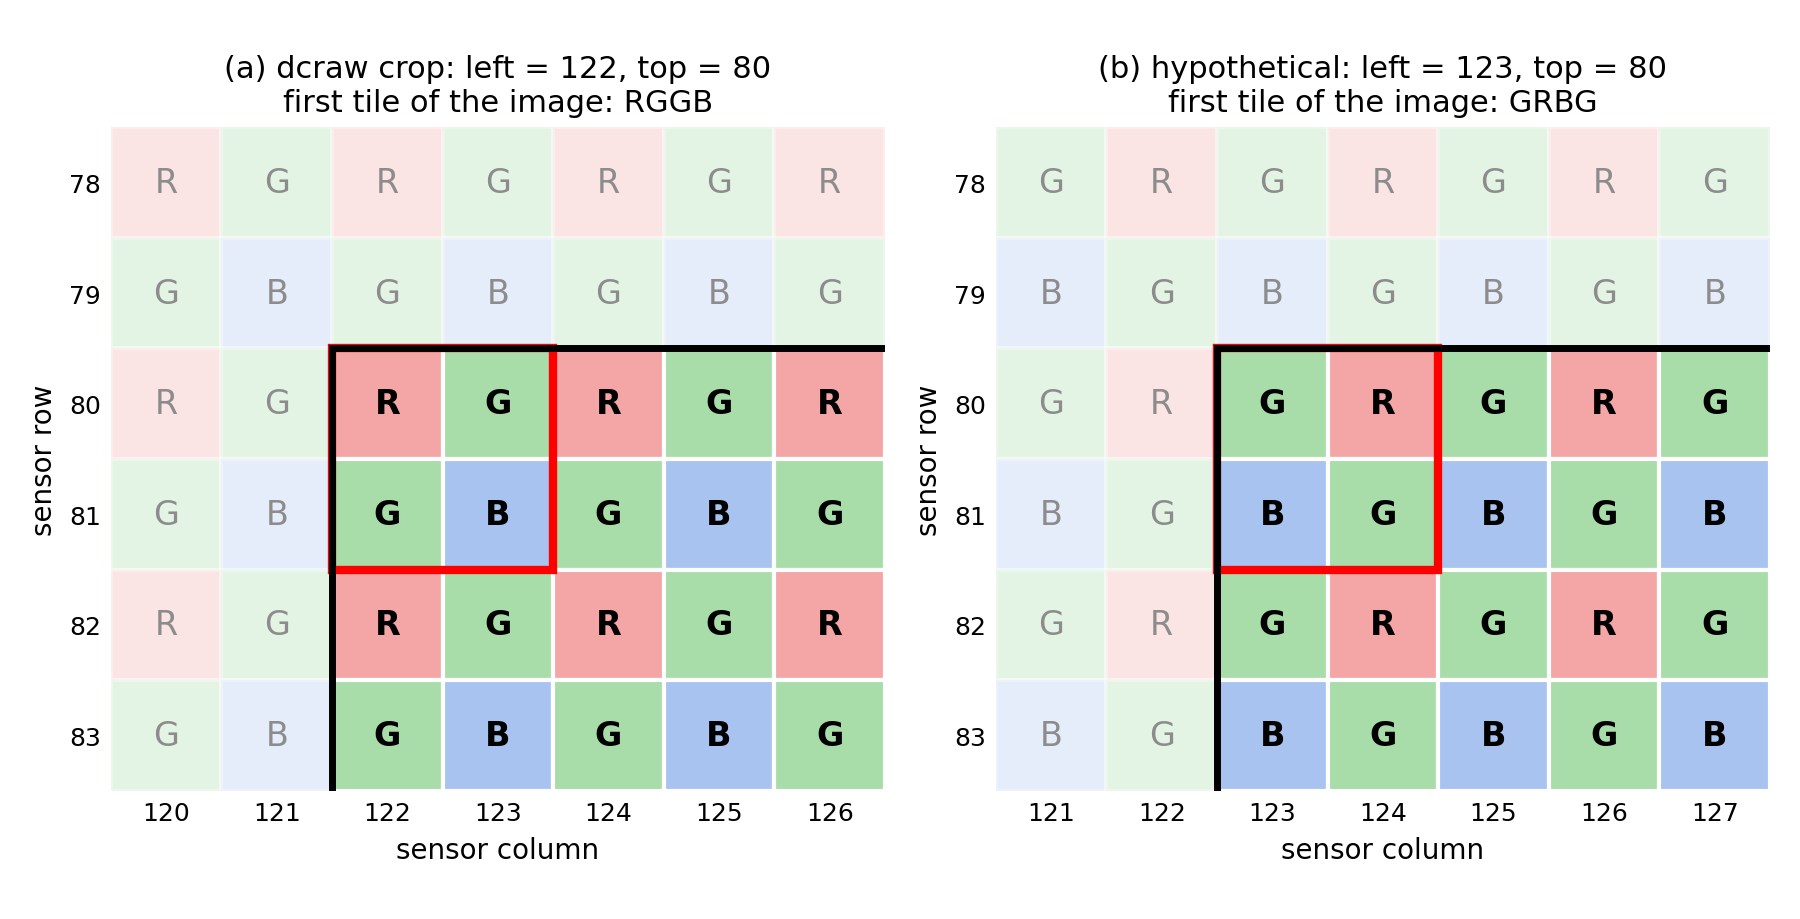
\includegraphics[width=0.72\textwidth]{figures/bayer_crop_parity.png}
    \caption{The color filter array of the sensor (from \texttt{filters = 0x94949494}) around the corner where the image starts. Faded pixels are cut away; the red square is the first $2 \times 2$ tile of the image. (a) The crop used by \texttt{dcraw} for \texttt{campus.tiff}. (b) A crop starting one column further right would change the pattern to \texttt{GRBG}.}
    \label{fig:crop_parity}
\end{figure}

\paragraph{Implementation.} The core of \texttt{detect\_bayer\_pattern\_from\_cr2()} (prints and error checks removed):
\begin{lstlisting}
CANON_FILTERS = 0x94949494
DCRAW_CANON_MARGINS = {(5920, 3950): (122, 80)}   # (left, top)

order = {b"II": "little", b"MM": "big"}.get(data[0:2])     # Step 1
def uint(offset, size):
    return int.from_bytes(data[offset:offset + size], order)
ifd0_offset, raw_ifd_offset = uint(4, 4), uint(12, 4)

def read_ifd(offset):                       # count + 12-byte entries
    n = uint(offset, 2)
    entries = {uint(e, 2): e + 8
               for e in range(offset + 2, offset + 2 + 12 * n, 12)}
    return entries, uint(offset + 2 + 12 * n, 4)

ifds, offset = [], ifd0_offset                             # Steps 2-3
while offset:
    entries, offset = read_ifd(offset)
    ifds.append(entries)
exif, _ = read_ifd(uint(ifds[0][0x8769], 4))
if any(tag in d for d in ifds + [exif] for tag in (0x828E, 0xA302)):
    raise ValueError("the file records its CFA layout")

raw_ifd, _ = read_ifd(raw_ifd_offset)                      # Step 4
pos = uint(raw_ifd[0x0111], 4) + 2          # skip SOI
while data[pos:pos + 2] != b"\xff\xc3":     # walk the JPEG markers
    pos += 2 + int.from_bytes(data[pos + 2:pos + 4], "big")
lines = int.from_bytes(data[pos + 5:pos + 7], "big")
samples = int.from_bytes(data[pos + 7:pos + 9], "big")
sensor_w, sensor_h = samples * data[pos + 9], lines

def sensor_color(row, col):                                # Step 5
    shift = (((row << 1) & 14) + (col & 1)) << 1
    return "RGB"[(CANON_FILTERS >> shift) & 3]

left, top = DCRAW_CANON_MARGINS[(sensor_w, sensor_h)]     # Step 6
makernote, _ = read_ifd(uint(exif[0x927C], 4))
sensor_info = uint(makernote[0x00E0], 4)    # SensorInfo
cam_left, cam_top = uint(sensor_info + 10, 2), uint(sensor_info + 12, 2)

def image_pattern(top, left):                              # Step 7
    return "".join(sensor_color(top + r, left + c)
                   for r in (0, 1) for c in (0, 1))
pattern = image_pattern(top, left)
self.pattern = pattern
\end{lstlisting}
Running it on \texttt{campus.CR2} prints:
\begin{lstlisting}[language={}, numbers=none]
--- Section 4.2.2: Bayer Pattern from the CR2 Bytes ---
Header: 49 49 2a 00 10 00 00 00 43 52 02 00 80 19 01 00
  byte order: little, IFD0 at 0x10, RAW IFD at 0x11980
Camera: Canon / Canon EOS 5D Mark III
CFAPattern tag (0x828E / 0xA302): not present -> CFA code 0x94949494
SOF3 at 0x411b1e: ff c3 00 0e 0e 0f 6e 0b 90 02
  14-bit, 3950 lines x 2960 samples x 2 components -> sensor 5920 x 3950
Sensor tile at (0, 0): RGGB
MakerNote SensorInfo (0x00E0): left 140, top 96 -> camera crop 5760 x 3840, pattern RGGB
Crop origin (left, top) = (122, 80) -> Bayer pattern: RGGB
\end{lstlisting}
The main block of \texttt{assign\_code.py} no longer hard-codes the Bayer pattern: it calls this method before \texttt{load\_raw\_tiff()}, and white balancing and demosaicing use the pattern read from the file. The result agrees with Strategy 1 and with \texttt{dcraw} itself, whose identification mode (\texttt{./dcraw -i -v campus.CR2}) reports \texttt{Filter pattern: RG/GB}.

\section{White Balancing}

\subsection{Implementation}
White balancing discounts the color of the ambient illuminant~\cite{ebner2007color} by scaling the Red and Blue channels relative to the Green channel ($s_g = 1.0$). The gains are applied to the Bayer mosaic itself, at the red and blue sites selected by the masks. I implemented four white balancing algorithms:
\begin{enumerate}
    \item \textbf{White World (Max-RGB):} Assumes the brightest value of each channel belongs to a white surface:
    \begin{equation}
        s_r = \frac{\max(G)}{\max(R)}, \quad s_b = \frac{\max(G)}{\max(B)}
    \end{equation}
    \item \textbf{Gray World:} Assumes the average spectral reflectance across the scene is achromatic gray:
    \begin{equation}
        s_r = \frac{\text{mean}(G)}{\text{mean}(R)}, \quad s_b = \frac{\text{mean}(G)}{\text{mean}(B)}
    \end{equation}
    \item \textbf{Camera Presets:} Uses the multipliers recorded by the camera and reported by \texttt{dcraw}:
    \begin{equation}
        s_r = \frac{m_1}{m_2} = \frac{1.858398}{1.0} \approx 1.8584, \quad s_b = \frac{m_3}{m_2} = \frac{1.723633}{1.0} \approx 1.7236
    \end{equation}
    \item \textbf{Manual White Balance:} Computed from a user-selected neutral patch ($[y_1:y_2, x_1:x_2]$):
    \begin{equation}
        s_r = \frac{\bar{G}_{\text{patch}}}{\bar{R}_{\text{patch}}}, \quad s_b = \frac{\bar{G}_{\text{patch}}}{\bar{B}_{\text{patch}}}
    \end{equation}
\end{enumerate}

\begin{lstlisting}
def white_balance(self, method='camera', manual_region=None):
    img = self.linear_image.copy()
    h, w = img.shape
    mask_r, mask_g, mask_b = self._build_bayer_masks(h, w, self.pattern)

    if method == 'white_world':
        s_r = img[mask_g].max() / img[mask_r].max()
        s_b = img[mask_g].max() / img[mask_b].max()
    elif method == 'gray_world':
        s_r = img[mask_g].mean() / img[mask_r].mean()
        s_b = img[mask_g].mean() / img[mask_b].mean()
    elif method == 'camera':
        s_r, s_b = self.wb_mults[0] / self.wb_mults[1], self.wb_mults[2] / self.wb_mults[1]
    elif method == 'manual':
        if manual_region is None:
            manual_region = (2400, 2450, 2800, 2850)
        y1, y2, x1, x2 = manual_region
        patch = img[y1:y2, x1:x2]
        s_r = patch[mask_g[y1:y2, x1:x2]].mean() / patch[mask_r[y1:y2, x1:x2]].mean()
        s_b = patch[mask_g[y1:y2, x1:x2]].mean() / patch[mask_b[y1:y2, x1:x2]].mean()

    img[mask_r] *= s_r
    img[mask_b] *= s_b
    self.linear_image = np.clip(img, 0.0, 1.0)
    return self.linear_image
\end{lstlisting}

\subsection{Manual Details: the Selected Patch}
For Manual White Balance I selected a $50 \times 50$ pixel patch at rows $y \in [2400, 2450)$ and columns $x \in [2800, 2850)$ of the full-resolution image, i.e.\ \texttt{manual\_region = (2400, 2450, 2800, 2850)}. It lies on the white marble plaque of the stone monument, on the blank area directly below the English inscription, in the part of the plaque that is in shade. The marble is a neutral surface, and the patch is uniform and far from saturation. Before white balancing its mean linear values are $\bar{R} = 0.0353$, $\bar{G} = 0.0755$, $\bar{B} = 0.0501$, which gives the gains $s_r = \bar{G} / \bar{R} = 2.1419$ and $s_b = \bar{G} / \bar{B} = 1.5059$ (computed from the unrounded means). After Manual White Balance the patch becomes exactly neutral: $\bar{R} = \bar{G} = \bar{B} = 0.0755$.

Figure~\ref{fig:wb_patch} shows the patch on the Manual White Balance result: (a) marks its position with a red square, and (b) shows the patch itself enlarged, which is now a neutral gray.

\begin{figure}[H]
    \centering
    \begin{subfigure}[b]{0.62\textwidth}
        \centering
        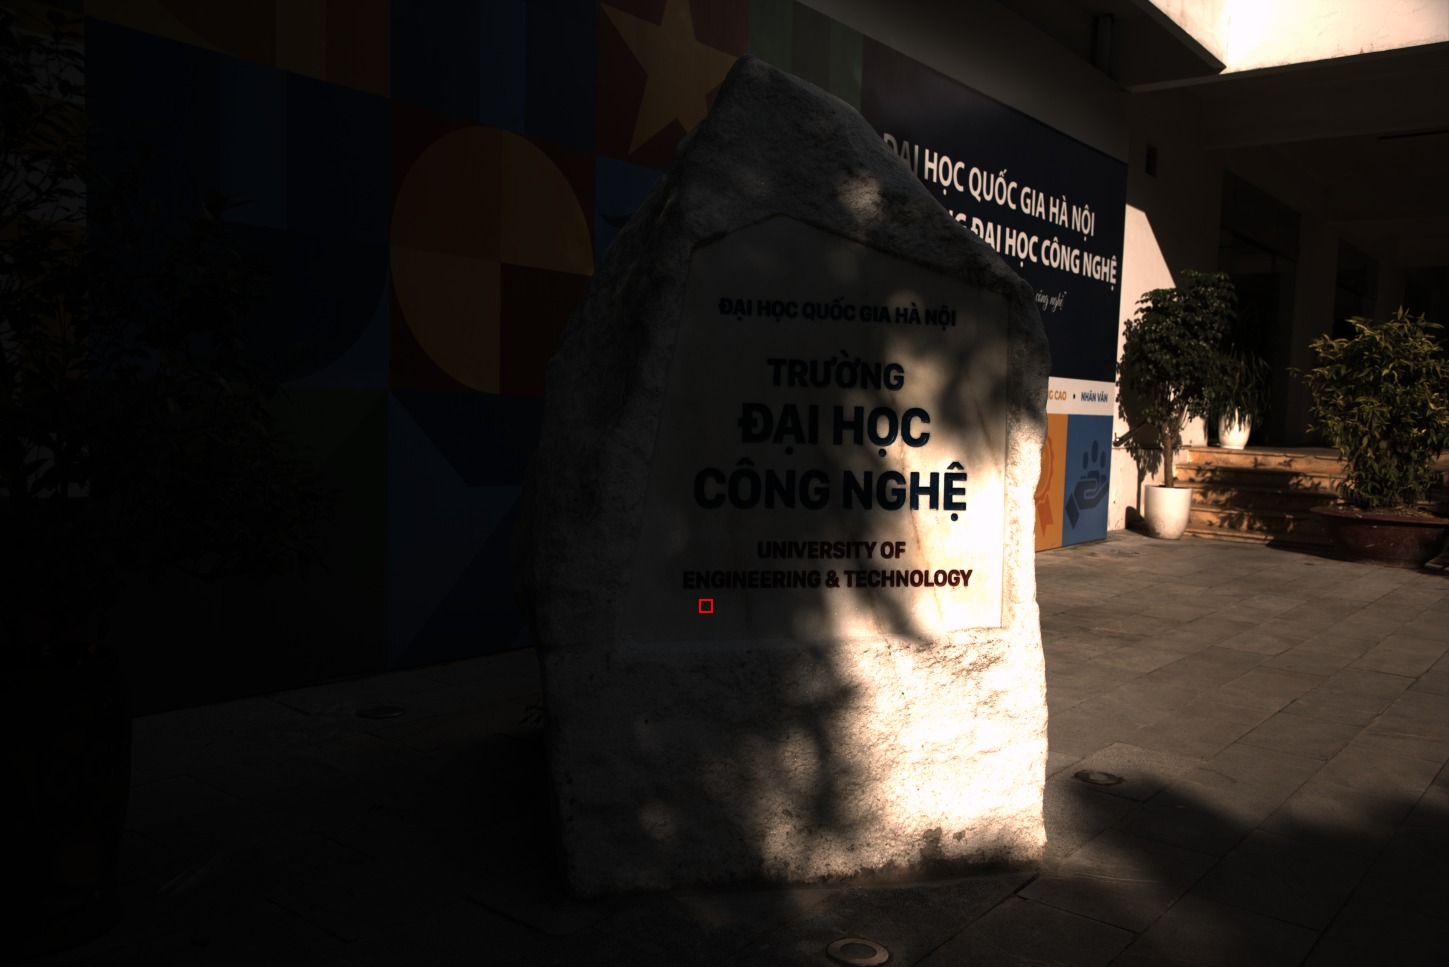
\includegraphics[width=\textwidth]{figures/wb_patch_location.jpg}
        \caption{Patch location (red square)}
        \label{fig:wb_patch_loc}
    \end{subfigure}
    \hfill
    \begin{subfigure}[b]{0.34\textwidth}
        \centering
        
\includegraphics[width=\textwidth]{figures/wb_patch_zoom.png}
        \caption{Patch zoom ($8\times$)}
        \label{fig:wb_patch_zoom}
    \end{subfigure}
    \caption{Selected patch for Manual White Balance, \texttt{manual\_region = (2400, 2450, 2800, 2850)}, shown on the Manual White Balance result. Image taken after the demosaicing step (linearization $\rightarrow$ manual white balancing $\rightarrow$ demosaicing, no color correction, brightness or gamma).}
    \label{fig:wb_patch}
\end{figure}

\subsection{Comparison}
Table~\ref{tab:wb_scalars} lists the gains computed by the four algorithms.

\begin{table}[H]
\centering
\caption{Calculated white balance scaling multipliers ($s_g = 1.0$)}
\label{tab:wb_scalars}
\begin{tabular}{lccc}
\toprule
\textbf{Method} & $\mathbf{s_r}$ & $\mathbf{s_g}$ & $\mathbf{s_b}$ \\
\midrule
White World (Max-RGB)    & $1.0155$ & $1.0000$ & $1.0155$ \\
Gray World               & $1.7070$ & $1.0000$ & $1.6979$ \\
Camera Presets           & $1.8584$ & $1.0000$ & $1.7236$ \\
Manual White Balance     & $2.1419$ & $1.0000$ & $1.5059$ \\
\bottomrule
\end{tabular}
\end{table}

Figure~\ref{fig:wb_comparison} shows the result of each method taken after the demosaicing step: linearization $\rightarrow$ white balancing $\rightarrow$ bilinear demosaicing (Section 6). Demosaicing is applied only so that the white-balanced mosaic can be displayed in color; no color correction, brightness scaling or gamma encoding is involved.

\begin{figure}[H]
    \centering
    \begin{subfigure}[b]{0.48\textwidth}
        \centering
        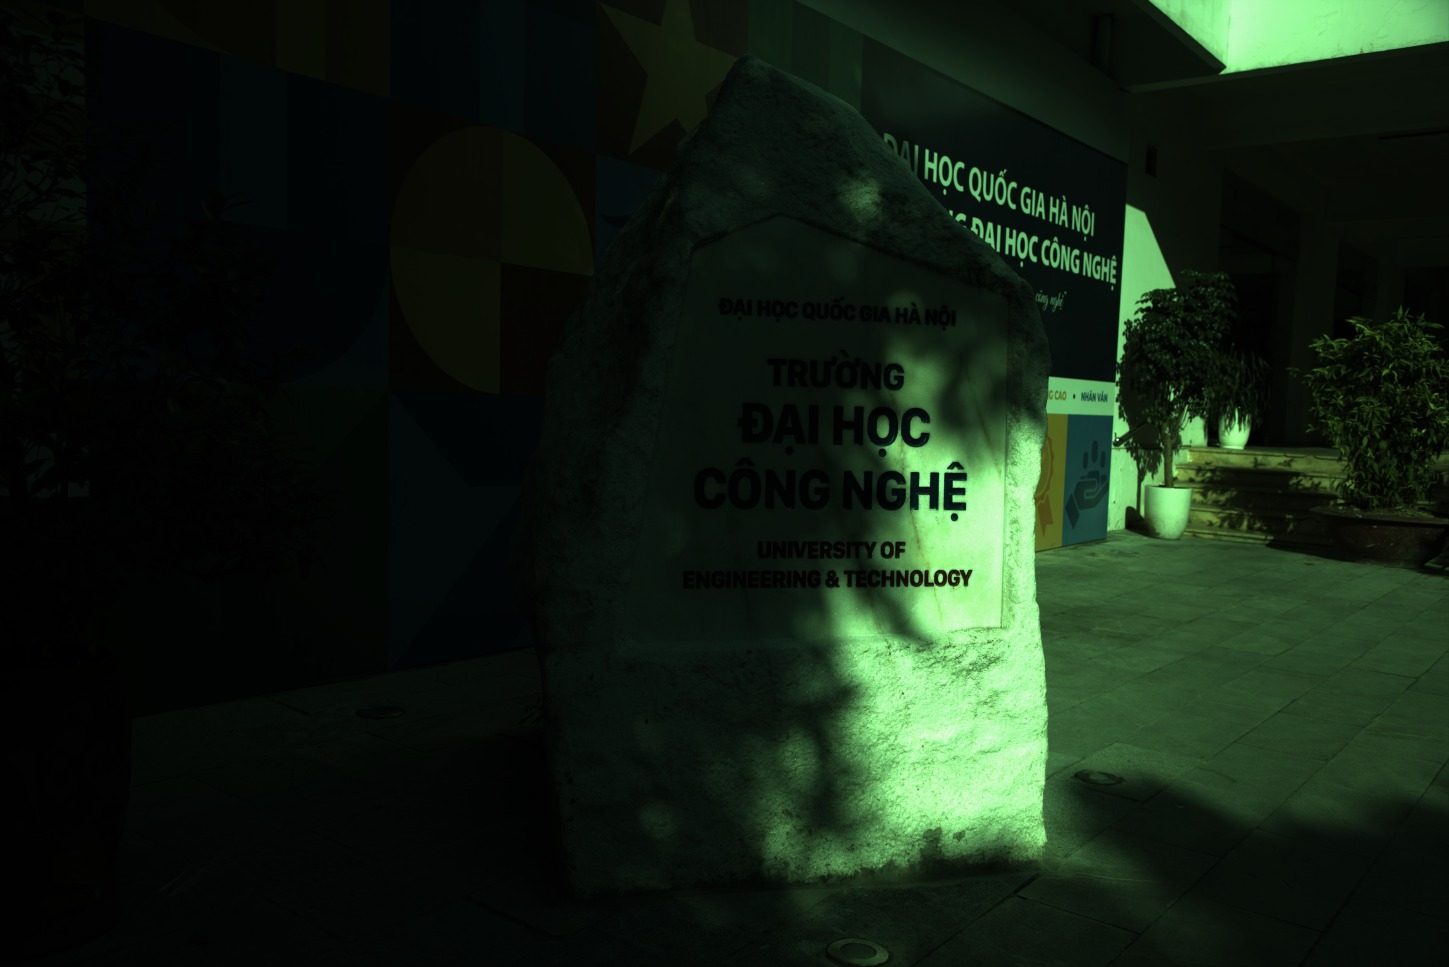
\includegraphics[width=\textwidth]{figures/wb_white_world.jpg}
        \caption{White World (Max-RGB)}
        \label{fig:wb_white}
    \end{subfigure}
    \hfill
    \begin{subfigure}[b]{0.48\textwidth}
        \centering
        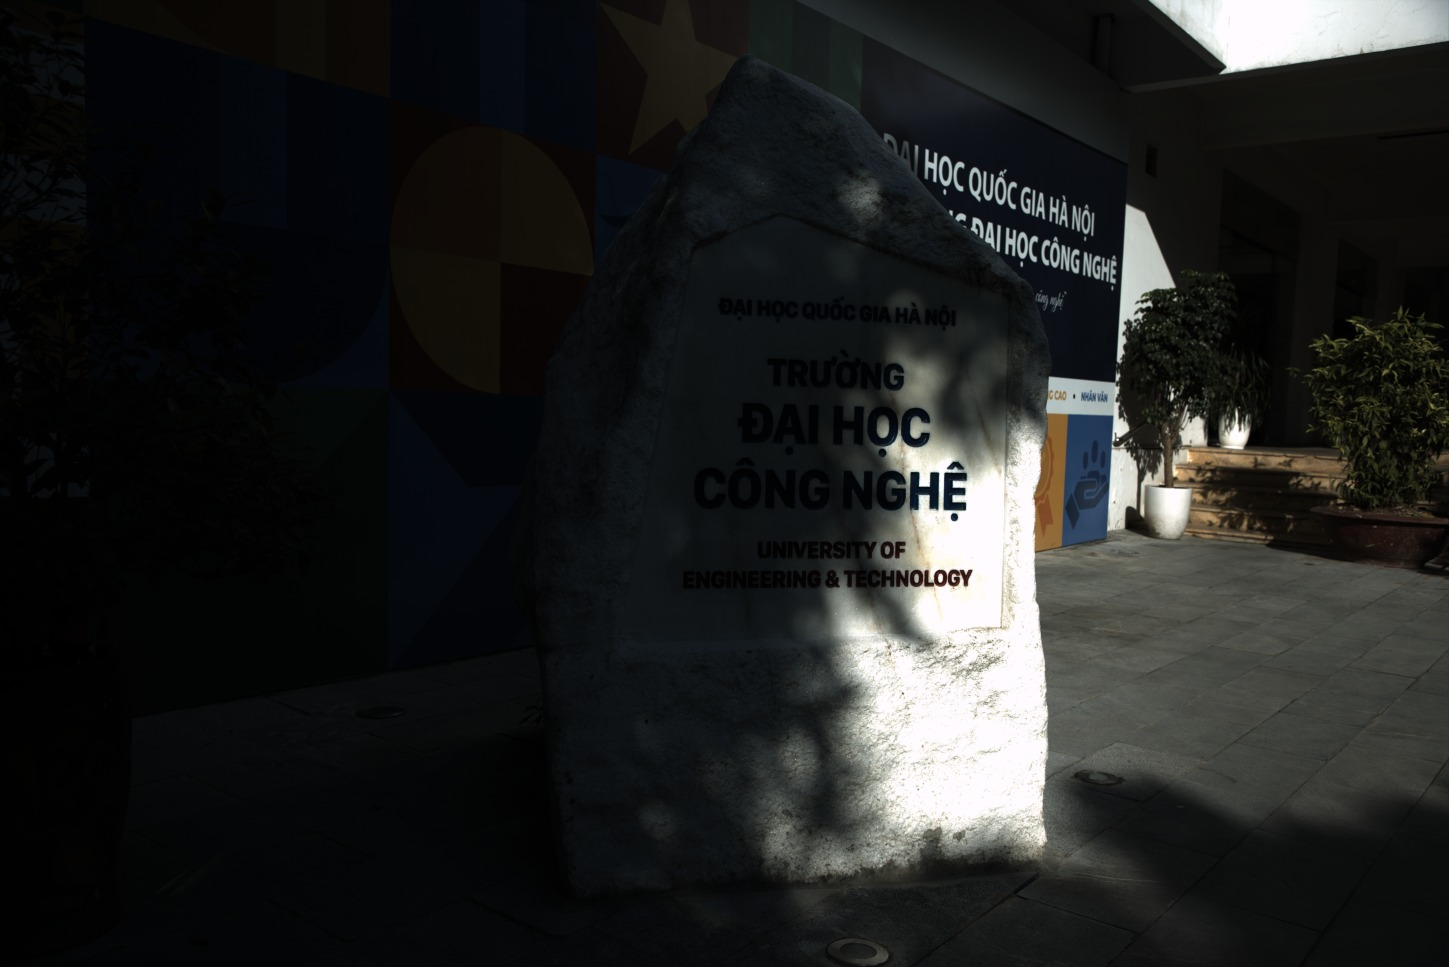
\includegraphics[width=\textwidth]{figures/wb_gray_world.jpg}
        \caption{Gray World}
        \label{fig:wb_gray}
    \end{subfigure}

    \vspace{0.3cm}
    \begin{subfigure}[b]{0.48\textwidth}
        \centering
        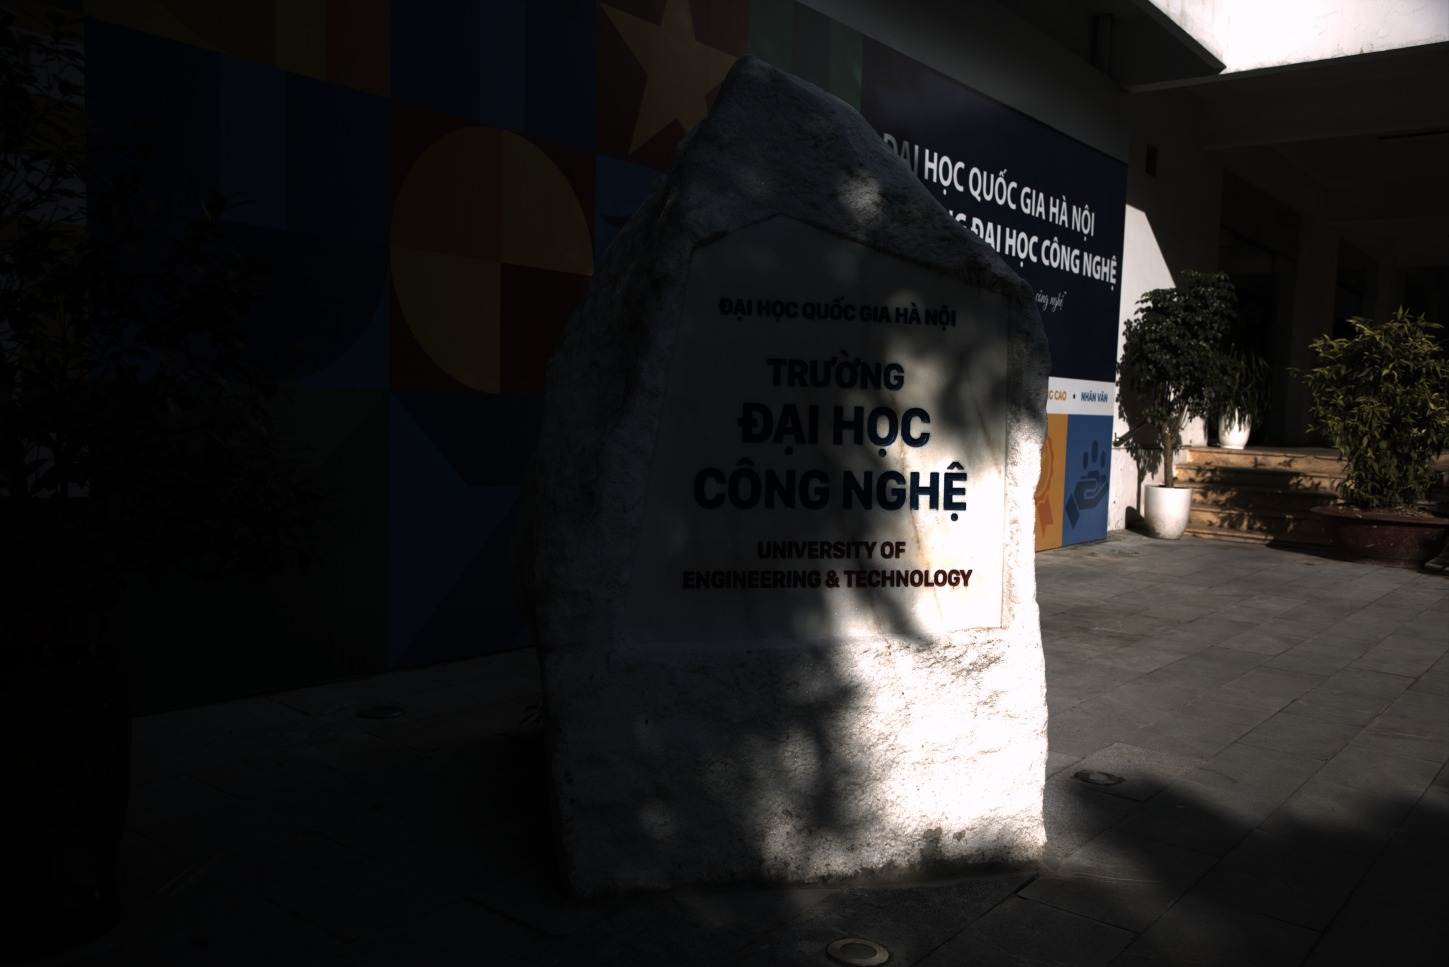
\includegraphics[width=\textwidth]{figures/wb_camera.jpg}
        \caption{Camera Presets}
        \label{fig:wb_camera}
    \end{subfigure}
    \hfill
    \begin{subfigure}[b]{0.48\textwidth}
        \centering
        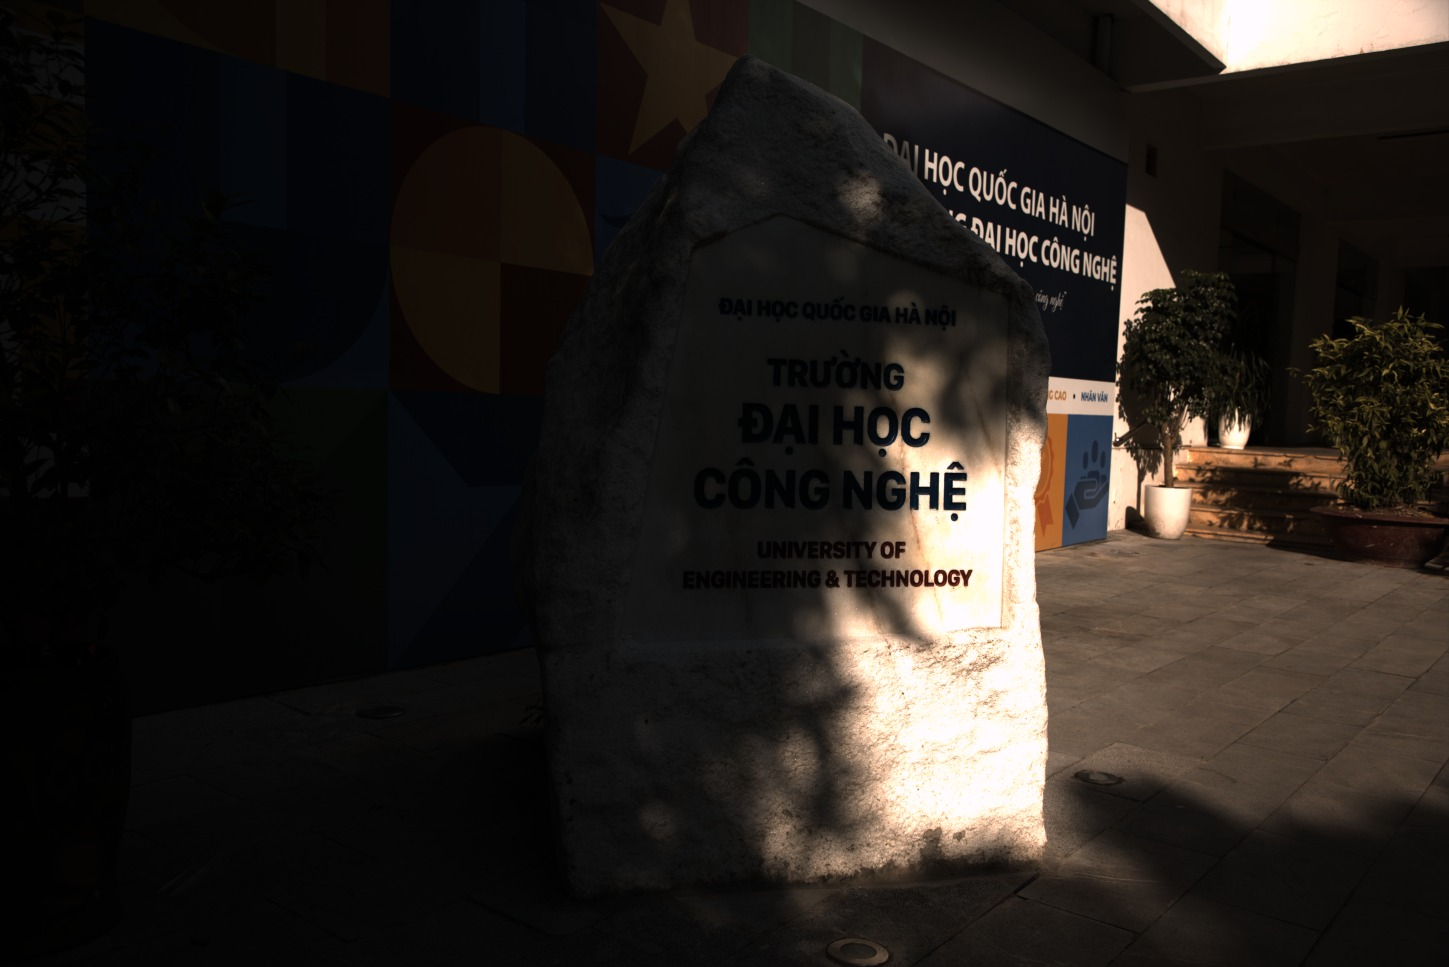
\includegraphics[width=\textwidth]{figures/wb_manual.jpg}
        \caption{Manual White Balance}
        \label{fig:wb_manual}
    \end{subfigure}
    \caption{The four white balancing methods. Images taken after the demosaicing step (linearization $\rightarrow$ white balancing $\rightarrow$ demosaicing, no color correction, brightness or gamma).}
    \label{fig:wb_comparison}
\end{figure}

\textbf{Comparative Analysis:}
\begin{itemize}
    \item \textbf{1. White World (Max-RGB):} This method performed the poorest. The overexposed area at the top right of the frame saturates all three channels, so the channel maxima are almost equal ($\max(R) = \max(B) = 0.9847$, $\max(G) = 1.0$) and the gains collapse to $s_r = s_b = 1.0155$. The image is left practically unbalanced and keeps the sensor's native green cast (Figure~\ref{fig:wb_white}). The ``brightest pixel is white'' assumption fails whenever the brightest pixels are clipped.
    \item \textbf{2. Gray World:} The gains ($s_r = 1.7070$, $s_b = 1.6979$) are close to the camera's, and the result is acceptable, but the red gain is about $8\%$ lower than the camera preset, which leaves a slightly cool, green-cyan tint on the white stone. The scene average is not gray: a large part of the frame is covered by the blue and green panels of the mural and by plants.
    \item \textbf{3. Camera Presets:} This produced the most natural result ($s_r = 1.8584$, $s_b = 1.7236$). The sunlit stone and the pavement are neutral and no region shows an obvious cast. The multipliers were measured by the camera for this exposure and do not depend on the content of the scene, so they are not misled by clipped highlights or by a colorful background.
    \item \textbf{4. Manual White Balance:} The selected patch becomes exactly neutral, but the patch is in shade, where the light comes mainly from the blue sky rather than from the sun. Neutralizing it therefore requires a stronger red gain and a weaker blue gain ($s_r = 2.1419$, $s_b = 1.5059$), and the sunlit parts of the stone and the pavement turn noticeably warm (yellowish). The scene has two illuminants, and a single patch can only correct one of them; the result depends strongly on where the patch is taken.
\end{itemize}
For this scene the Camera Presets are therefore the best choice, and they are used for the rest of the pipeline.

\section{Demosaicing}

\subsection{Implementation}
Because each pixel of the Bayer mosaic records only one color channel, the two missing colors must be interpolated~\cite{malvar2004demosaicing}. In bilinear demosaicing a missing value is the average of the nearest measured samples of that color. Which neighbors hold such samples depends on the site, so four averaging kernels are needed. Each has a zero center and weights that sum to $1$:
\begin{equation}
    K_{\text{cross}} = \frac{1}{4}\begin{bmatrix} 0 & 1 & 0 \\ 1 & 0 & 1 \\ 0 & 1 & 0 \end{bmatrix}, \quad
    K_{\text{diag}} = \frac{1}{4}\begin{bmatrix} 1 & 0 & 1 \\ 0 & 0 & 0 \\ 1 & 0 & 1 \end{bmatrix}, \quad
    K_{\text{horiz}} = \frac{1}{2}\begin{bmatrix} 0 & 0 & 0 \\ 1 & 0 & 1 \\ 0 & 0 & 0 \end{bmatrix}, \quad
    K_{\text{vert}} = \frac{1}{2}\begin{bmatrix} 0 & 1 & 0 \\ 0 & 0 & 0 \\ 0 & 1 & 0 \end{bmatrix}
\end{equation}
\begin{itemize}
    \item \textbf{Green at a red or blue site:} the four cross neighbors are all green, so $K_{\text{cross}}$ is used.
    \item \textbf{Red at a blue site (and blue at a red site):} the four diagonal neighbors hold the wanted color, so $K_{\text{diag}}$ is used.
    \item \textbf{Red or blue at a green site:} only two neighbors hold the wanted color. They are the left and right neighbors if the green site lies in a row that contains that color ($K_{\text{horiz}}$), and the upper and lower neighbors otherwise ($K_{\text{vert}}$).
    \item \textbf{Measured samples} are copied unchanged.
\end{itemize}
Each kernel is applied with \texttt{scipy.ndimage.convolve} to the sparse channel (the mosaic multiplied by the channel mask, so that pixels of other colors contribute zero), and its result is used only at the sites it is meant for. The borders use \texttt{mode="mirror"}, which reflects about the center of the edge pixel and therefore keeps the Bayer phase intact outside the image.

\begin{lstlisting}
def demosaic_bilinear(self):
    img = self.linear_image
    h, w = img.shape
    mask_r, mask_g, mask_b = self._build_bayer_masks(h, w, self.pattern)

    k_cross = np.array([[0, 1, 0], [1, 0, 1], [0, 1, 0]]) / 4.0
    k_diag  = np.array([[1, 0, 1], [0, 0, 0], [1, 0, 1]]) / 4.0
    k_horiz = np.array([[0, 0, 0], [1, 0, 1], [0, 0, 0]]) / 2.0
    k_vert  = np.array([[0, 1, 0], [0, 0, 0], [0, 1, 0]]) / 2.0

    g_sparse = img * mask_g
    g_channel = np.where(mask_g, img, convolve(g_sparse, k_cross, mode="mirror"))

    def interpolate_red_or_blue(mask_c, mask_opposite):
        sparse = img * mask_c
        rows_with_c = mask_c.any(axis=1, keepdims=True)
        g_same_row = mask_g & rows_with_c
        g_other_row = mask_g & ~rows_with_c

        channel = sparse.copy()
        channel[mask_opposite] = convolve(sparse, k_diag, mode="mirror")[mask_opposite]
        channel[g_same_row] = convolve(sparse, k_horiz, mode="mirror")[g_same_row]
        channel[g_other_row] = convolve(sparse, k_vert, mode="mirror")[g_other_row]
        return channel

    r_channel = interpolate_red_or_blue(mask_r, mask_b)
    b_channel = interpolate_red_or_blue(mask_b, mask_r)

    self.rgb_linear = np.clip(np.stack([r_channel, g_channel, b_channel], axis=-1), 0.0, 1.0)
    return self.rgb_linear
\end{lstlisting}

\subsection{Comparison}
Figure~\ref{fig:demosaic_channels} displays the resulting Red, Green, and Blue channels of the image directly after bilinear demosaicing, rendered in their respective primary color planes.

\begin{figure}[H]
    \centering
    \begin{subfigure}[b]{0.32\textwidth}
        \centering
        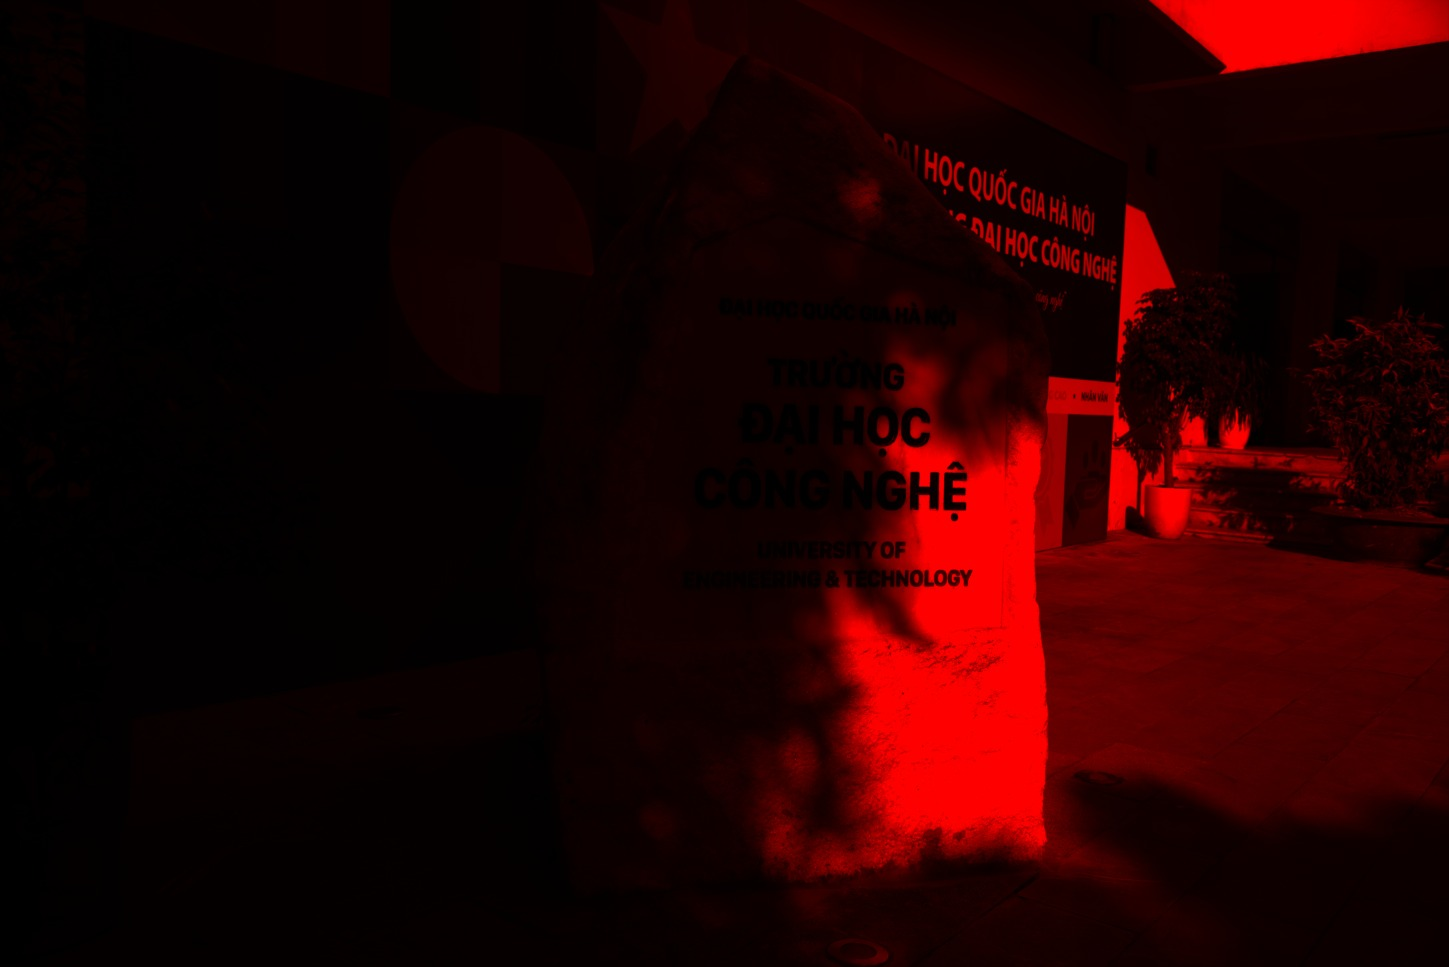
\includegraphics[width=\textwidth]{figures/channel_red.jpg}
        \caption{Red channel}
        \label{fig:ch_red}
    \end{subfigure}
    \hfill
    \begin{subfigure}[b]{0.32\textwidth}
        \centering
        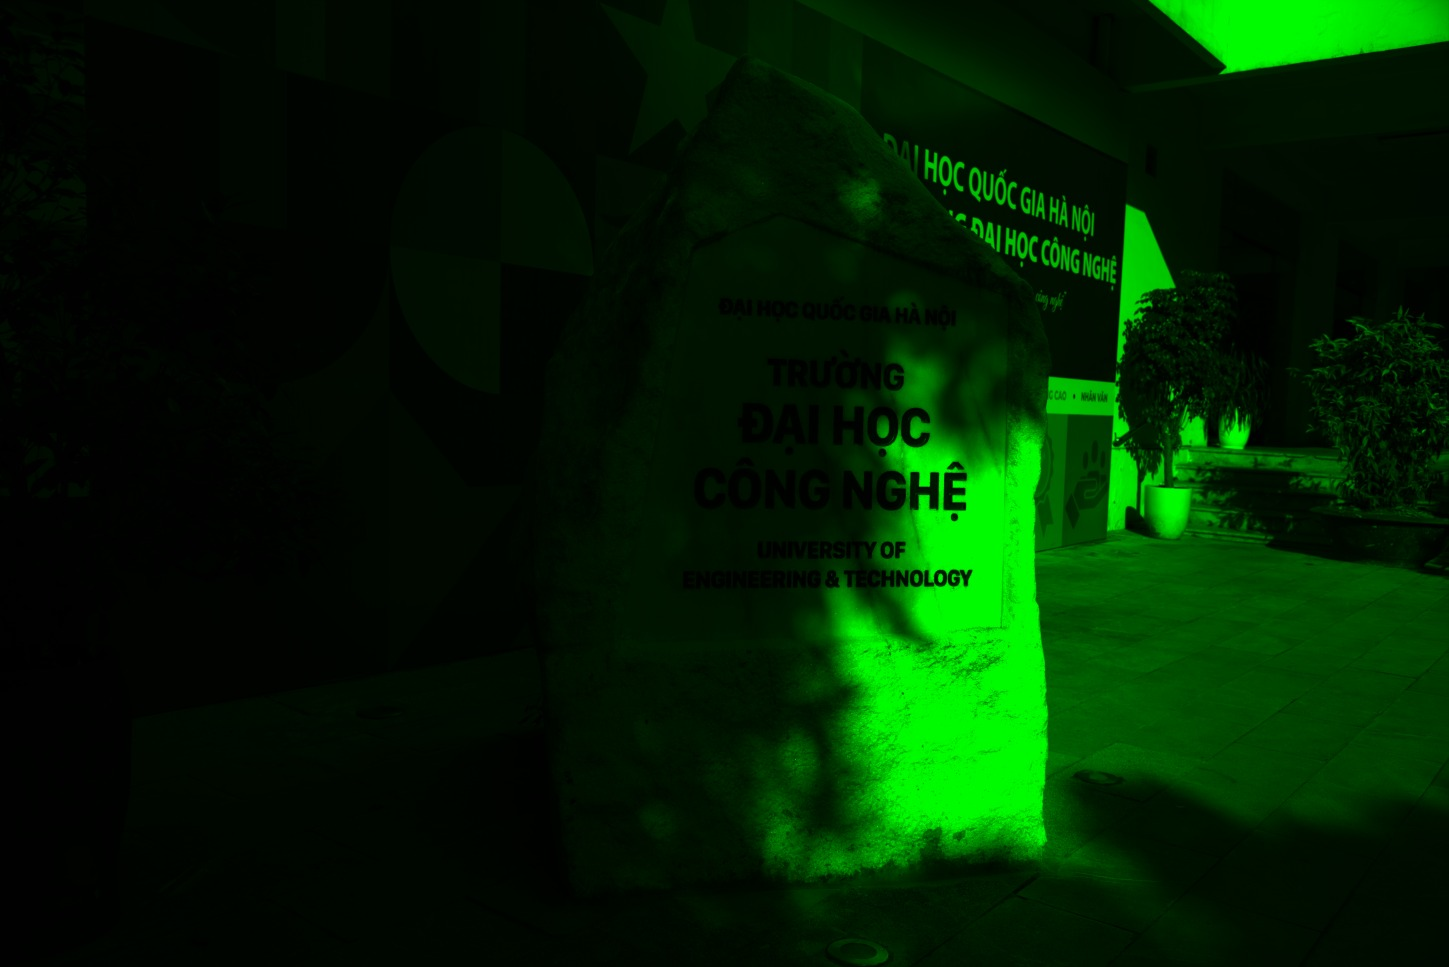
\includegraphics[width=\textwidth]{figures/channel_green.jpg}
        \caption{Green channel}
        \label{fig:ch_green}
    \end{subfigure}
    \hfill
    \begin{subfigure}[b]{0.32\textwidth}
        \centering
        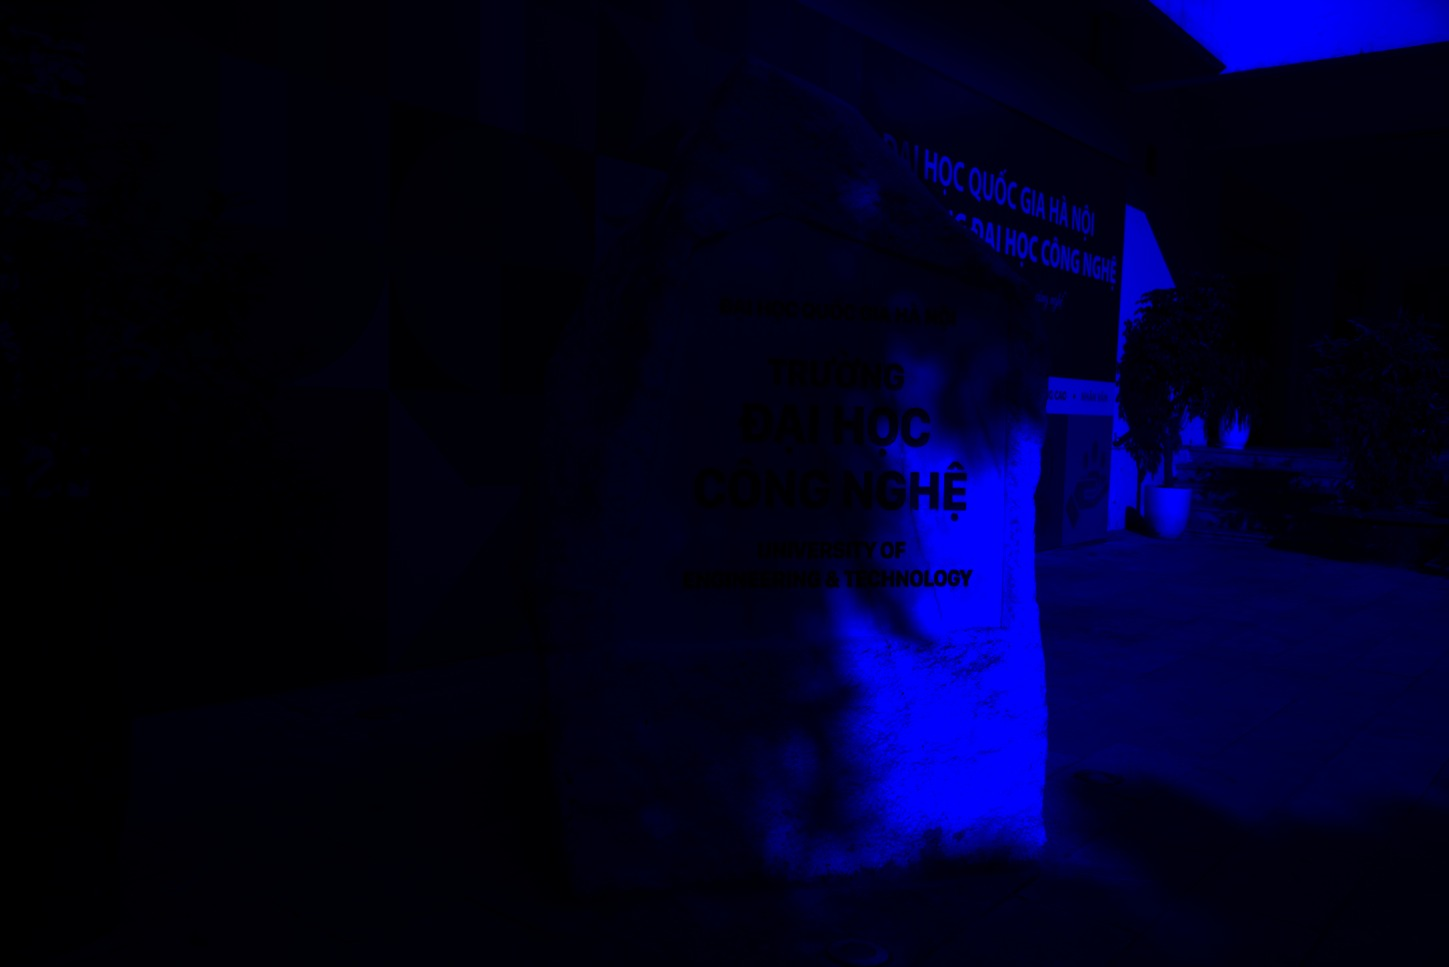
\includegraphics[width=\textwidth]{figures/channel_blue.jpg}
        \caption{Blue channel}
        \label{fig:ch_blue}
    \end{subfigure}
    \caption{The individual R, G, and B channels directly after bilinear demosaicing (rendered in their respective primary color planes).}
    \label{fig:demosaic_channels}
\end{figure}

A full-frame view is reduced too much to show individual pixels, so Figure~\ref{fig:demosaic_crop} enlarges a $32 \times 32$ pixel window (rows $2464$--$2495$, columns $3368$--$3399$, on the sunlit marble of the plaque just below the inscription, where no value is clipped), each channel drawn in its own color. Before interpolation (top row) a channel holds values only at its own Bayer sites, and the unmeasured sites, shown in white, form a regular grid: $768$ of the $1024$ pixels are empty for red and blue and $512$ for green, which gives the checkerboard. After interpolation (bottom row) every pixel has a value, none of them is zero, and the grid has disappeared.

\begin{figure}[H]
    \centering
    \begin{subfigure}[b]{0.22\textwidth}
        \centering
        
\includegraphics[width=\textwidth]{figures/crop_sparse_red.png}
        \caption{Red, before}
    \end{subfigure}
    \hspace{0.04\textwidth}
    \begin{subfigure}[b]{0.22\textwidth}
        \centering
        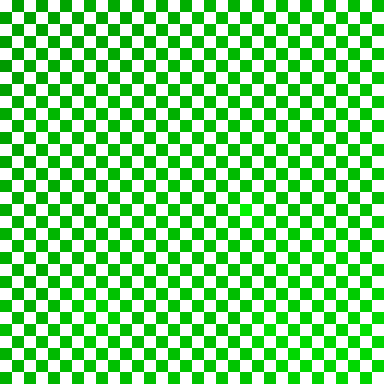
\includegraphics[width=\textwidth]{figures/crop_sparse_green.png}
        \caption{Green, before}
    \end{subfigure}
    \hspace{0.04\textwidth}
    \begin{subfigure}[b]{0.22\textwidth}
        \centering
        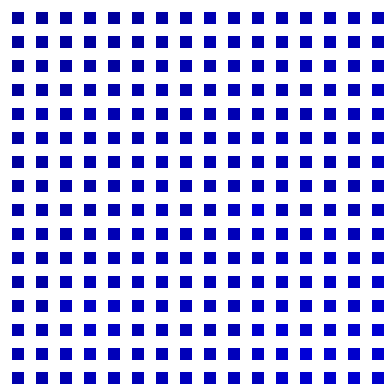
\includegraphics[width=\textwidth]{figures/crop_sparse_blue.png}
        \caption{Blue, before}
    \end{subfigure}

    \vspace{0.2cm}
    \begin{subfigure}[b]{0.22\textwidth}
        \centering
        
\includegraphics[width=\textwidth]{figures/crop_dense_red.png}
        \caption{Red, after}
    \end{subfigure}
    \hspace{0.04\textwidth}
    \begin{subfigure}[b]{0.22\textwidth}
        \centering
        
\includegraphics[width=\textwidth]{figures/crop_dense_green.png}
        \caption{Green, after}
    \end{subfigure}
    \hspace{0.04\textwidth}
    \begin{subfigure}[b]{0.22\textwidth}
        \centering
        
\includegraphics[width=\textwidth]{figures/crop_dense_blue.png}
        \caption{Blue, after}
    \end{subfigure}
    \caption{A $32 \times 32$ pixel window of each channel before (top) and after (bottom) bilinear demosaicing, enlarged $12\times$. White pixels in the top row are sites where the channel was not measured.}
    \label{fig:demosaic_crop}
\end{figure}

The three channels are dense and consistent with each other, which confirms that bilinear demosaicing reconstructs a complete RGB image from the Bayer mosaic.

\section{Color Space Correction}

\subsection{Implementation}
Raw camera sensor dyes do not correspond to the standard sRGB primaries. To map camera RGB coordinates to standard sRGB, the device-independent CIE XYZ 1931 space~\cite{cie1931} is used as an intermediate bridge:
\begin{equation}
    M_{\text{sRGB}\to\text{Cam}} = M_{\text{XYZ}\to\text{Cam}} \cdot M_{\text{sRGB}\to\text{XYZ}}
\end{equation}
\begin{equation}
    M_{\text{Cam}\to\text{sRGB}} = \left(M_{\text{sRGB}\to\text{Cam}}\right)^{-1}
\end{equation}
Using the Canon EOS 5D Mark III sensor matrix from the \texttt{adobe\_coeff} table of \texttt{dcraw} and the standard $M_{\text{sRGB}\to\text{XYZ}}$ matrix~\cite{iec1999srgb}:
\begin{equation}
    M_{\text{XYZ}\to\text{Cam}} = \frac{1}{10000}\begin{bmatrix} 6722 & -635 & -963 \\ -4287 & 12460 & 2028 \\ -908 & 2162 & 5668 \end{bmatrix}
\end{equation}
\begin{equation}
    M_{\text{sRGB}\to\text{XYZ}} = \begin{bmatrix} 0.4124564 & 0.3575761 & 0.1804375 \\ 0.2126729 & 0.7151522 & 0.0721750 \\ 0.0193339 & 0.1191920 & 0.9503041 \end{bmatrix}
\end{equation}
their product is
\begin{equation}
    M_{\text{sRGB}\to\text{Cam}} = \begin{bmatrix}
    0.26188661 & 0.18347230 & 0.02519269 \\
    0.09209129 & 0.76195890 & 0.20529817 \\
    0.01948729 & 0.18970602 & 0.53785287
    \end{bmatrix},
    \qquad \text{row sums: } \begin{bmatrix} 0.47055160 \\ 1.05934836 \\ 0.74704619 \end{bmatrix}
    \label{eq:srgb2cam}
\end{equation}
The rows of $M_{\text{sRGB}\to\text{Cam}}$ must be normalized before the matrix is inverted: each row is divided by its sum, so that every row sums to $1$, and the normalized matrix is then inverted (see Section~\ref{sec:norm_order}). The final matrix applied to every pixel is
\begin{equation}
    M_{\text{Cam}\to\text{sRGB}} = \begin{bmatrix}
     1.96439218 & -1.11971110 &  0.15531892 \\
    -0.24116035 &  1.67375571 & -0.43259536 \\
     0.01388648 & -0.54978120 &  1.53589472
    \end{bmatrix}
    \label{eq:cam2srgb}
\end{equation}

\begin{lstlisting}
def color_space_correction(self, M_xyz_to_cam):
    M_srgb_to_xyz = np.array([
        [0.4124564, 0.3575761, 0.1804375],
        [0.2126729, 0.7151522, 0.0721750],
        [0.0193339, 0.1191920, 0.9503041]
    ])
    M_srgb_to_cam = M_xyz_to_cam @ M_srgb_to_xyz
    # normalize rows first, then invert
    M_srgb_to_cam = M_srgb_to_cam / M_srgb_to_cam.sum(axis=1, keepdims=True)
    M_cam_to_srgb = np.linalg.inv(M_srgb_to_cam)

    h, w, c = self.rgb_linear.shape
    flat_rgb = self.rgb_linear.reshape(-1, 3)
    corrected_flat = flat_rgb @ M_cam_to_srgb.T
    self.rgb_linear = np.clip(corrected_flat.reshape(h, w, c), 0.0, 1.0)
    return self.rgb_linear
\end{lstlisting}

\subsection{Row Normalization}
\label{sec:norm_order}
\textbf{The rows of $M_{\text{sRGB}\to\text{Cam}}$ must be normalized before the matrix is inverted.} The image entering this stage has already been white balanced, so a white surface in it has the camera value $[1, 1, 1]^T$. When every row of $M_{\text{sRGB}\to\text{Cam}}$ sums to $1$, sRGB white $[1, 1, 1]^T$ corresponds to exactly this camera white, and the inverse matrix maps camera white back to sRGB white: the rows of $M_{\text{Cam}\to\text{sRGB}}$ in Eq.~\eqref{eq:cam2srgb} also sum to $1$.

Figure~\ref{fig:cc_norm} shows the same demosaiced image converted without and with the normalization. Without it, the rows of the inverted matrix sum to $[3.33, 0.49, 1.57]$ instead of $[1, 1, 1]$, so red is amplified and green is suppressed: the white stone and the gray pavement turn pink and the whole image has a strong magenta cast. With the normalization the stone and the pavement stay neutral and the colors of the mural and the plants are natural.

\begin{figure}[H]
    \centering
    \begin{subfigure}[b]{0.48\textwidth}
        \centering
        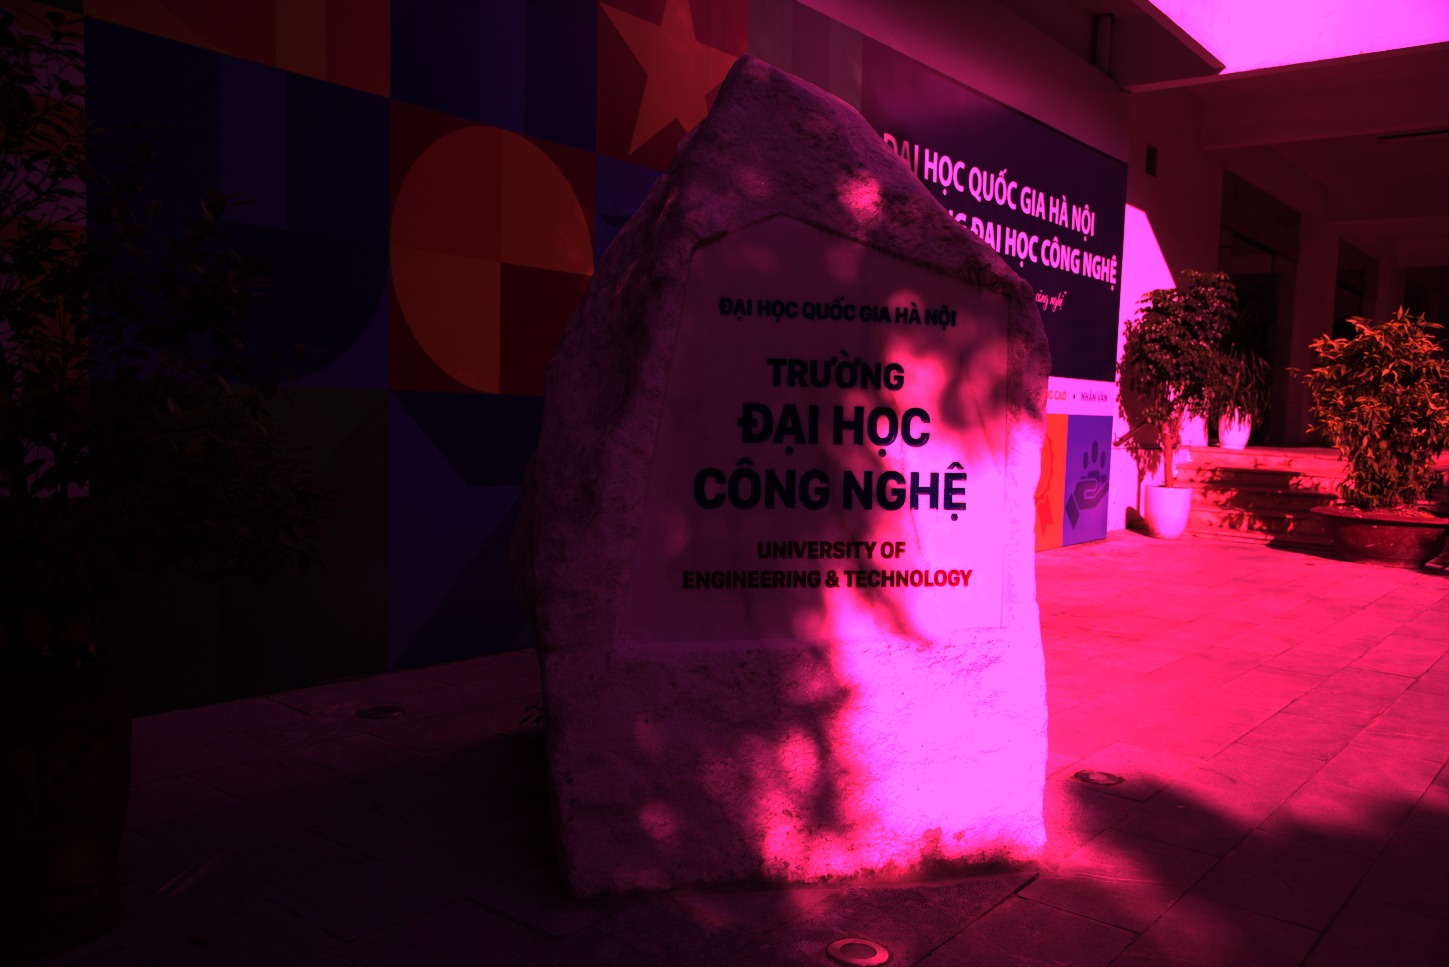
\includegraphics[width=\textwidth]{figures/cc_no_norm.jpg}
        \caption{Without normalization}
        \label{fig:cc_none}
    \end{subfigure}
    \hfill
    \begin{subfigure}[b]{0.48\textwidth}
        \centering
        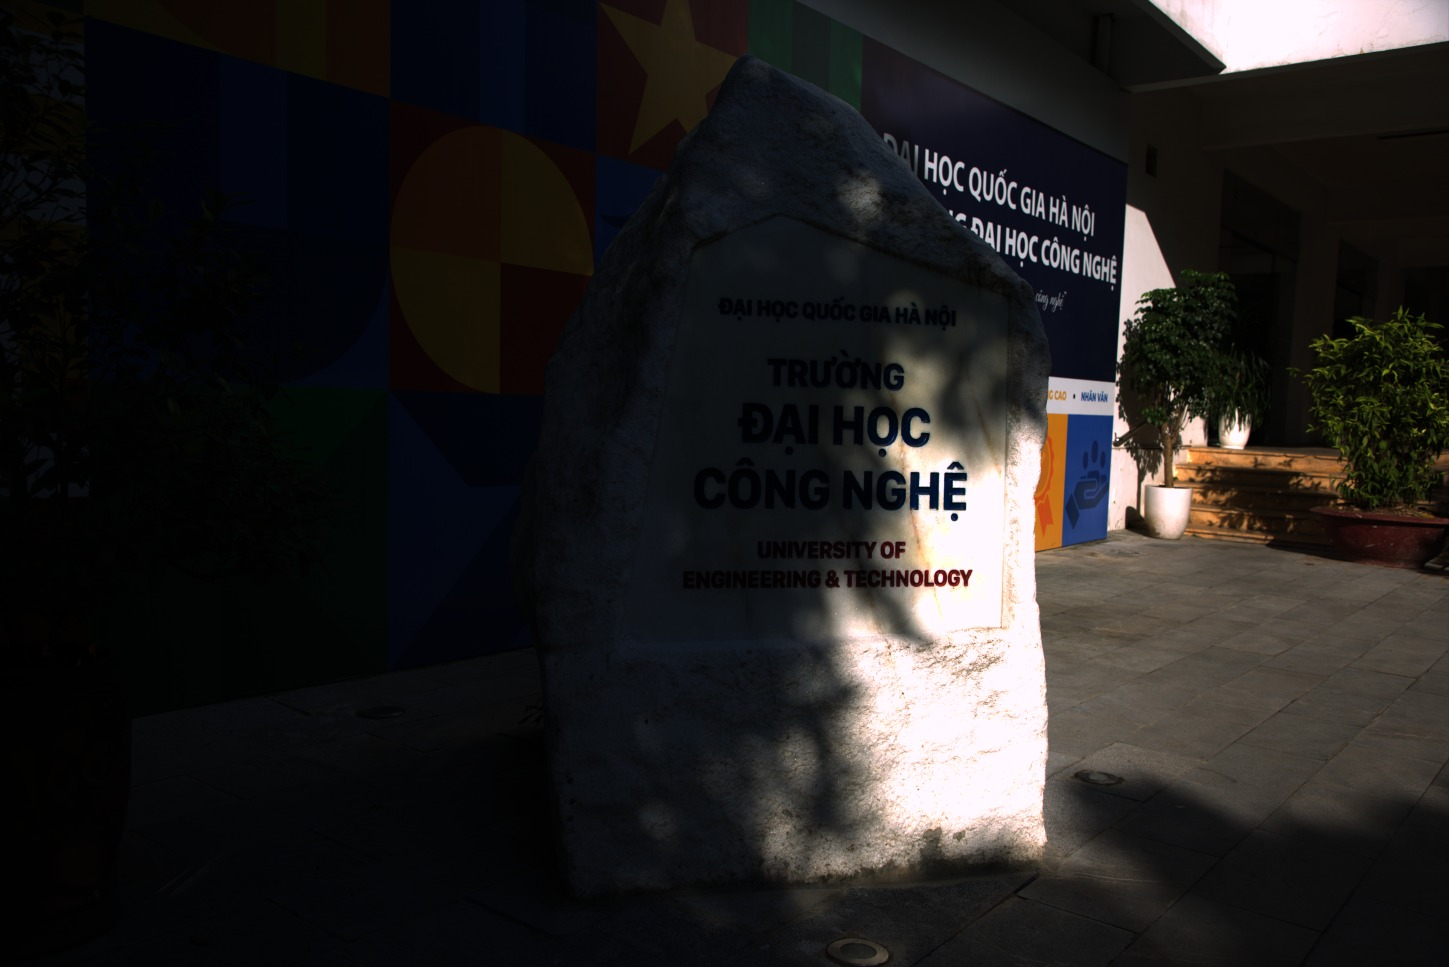
\includegraphics[width=\textwidth]{figures/cc_with_norm.jpg}
        \caption{With normalization before the inversion}
        \label{fig:cc_with_norm}
    \end{subfigure}
    \caption{Effect of normalizing the rows of $M_{\text{sRGB}\to\text{Cam}}$ before inverting it. Images taken after the color space correction step, no brightness or gamma.}
    \label{fig:cc_norm}
\end{figure}

\subsection{Comparison}
Figure~\ref{fig:color_correction_comp} displays the image immediately before and immediately after color space correction, rendered directly at this pipeline stage in pure linear radiance (without applying the subsequent brightness scaling and non-linear gamma encoding of Section 8).

\begin{figure}[H]
    \centering
    \begin{subfigure}[b]{0.48\textwidth}
        \centering
        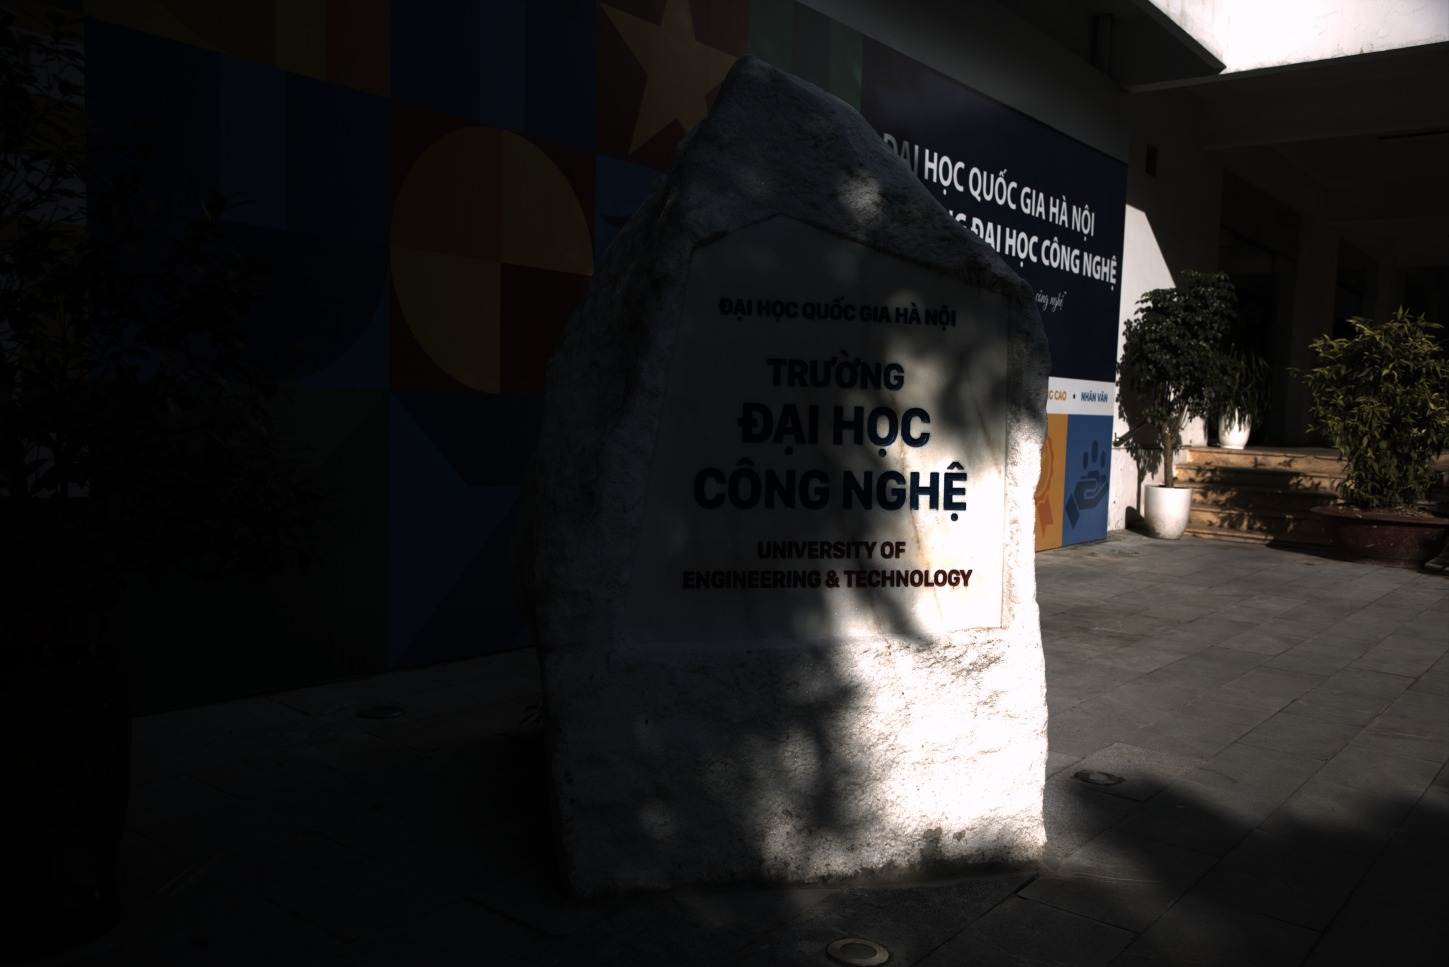
\includegraphics[width=\textwidth]{figures/color_corr_before.jpg}
        \caption{Before color correction (linear camera RGB)}
        \label{fig:cc_before}
    \end{subfigure}
    \hfill
    \begin{subfigure}[b]{0.48\textwidth}
        \centering
        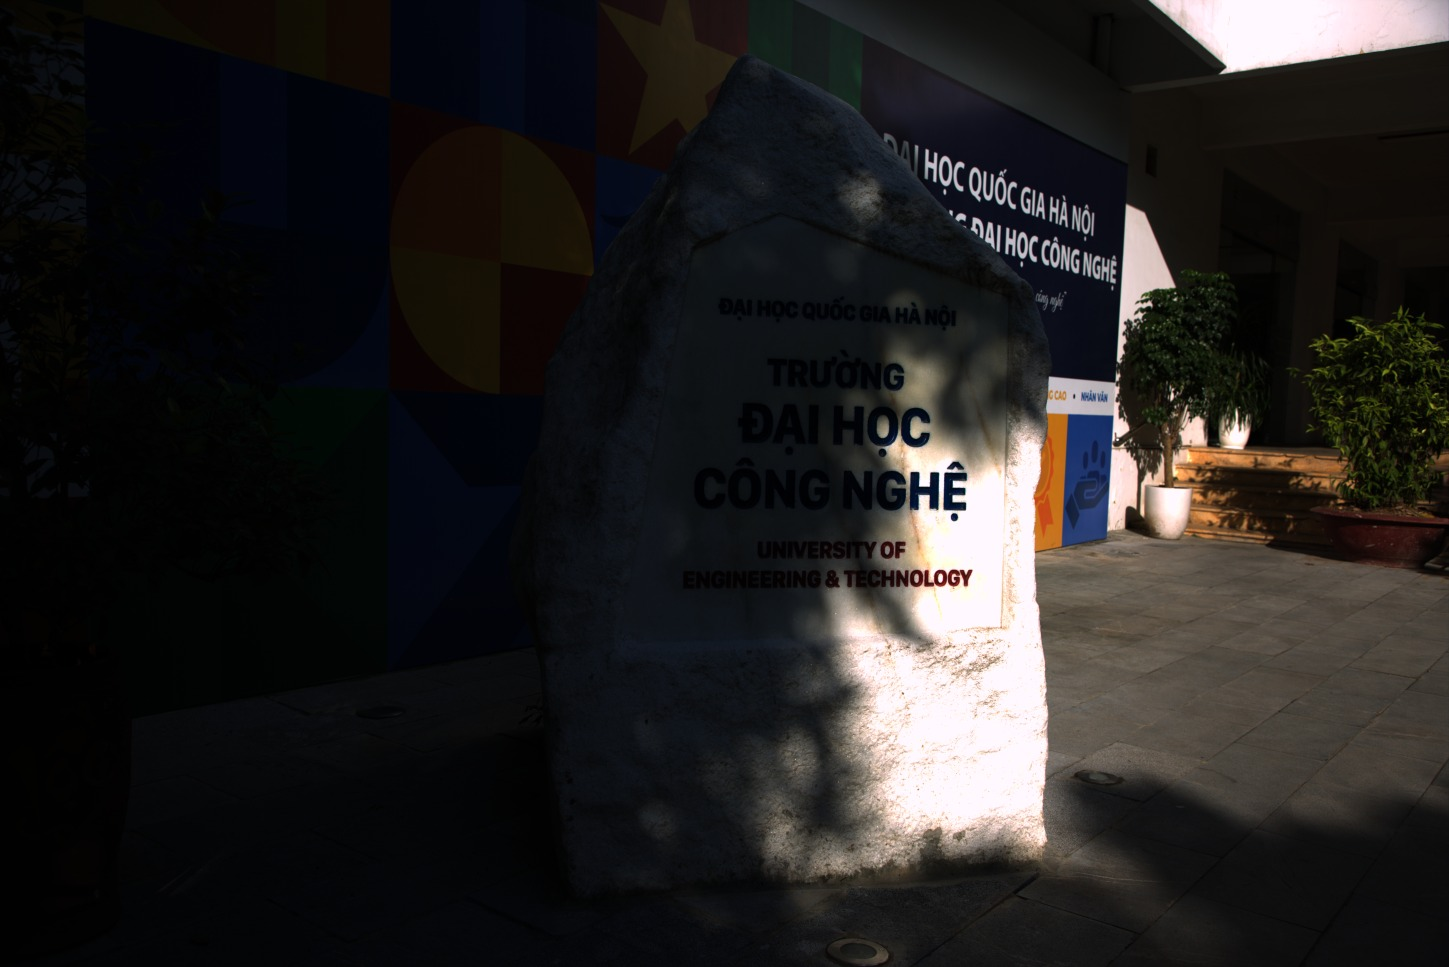
\includegraphics[width=\textwidth]{figures/color_corr_after.jpg}
        \caption{After color correction (linear sRGB)}
        \label{fig:cc_after}
    \end{subfigure}
    \caption{Visual comparison before and after Color Space Correction. Images taken directly before and after the color space correction step, no brightness or gamma.}
    \label{fig:color_correction_comp}
\end{figure}

\textbf{Visual Analysis:}
\begin{itemize}
    \item \textbf{Before Color Space Correction (Figure~\ref{fig:cc_before}):} The pixels reside in camera-native RGB space. Because the sensor spectral sensitivities differ from standard display phosphor/LCD primaries, chromaticities appear muted, muddy, and desaturated (e.g., foliage has an unnatural olive-yellow cast, and the mural panels appear dull).
    \item \textbf{After Color Space Correction (Figure~\ref{fig:cc_after}):} Applying the matrix $M_{\text{Cam}\to\text{sRGB}}$ maps the camera coordinates into the standardized sRGB color space. Foliage shifts into true green chromaticities, the inscription becomes clearly red, and the blue, orange and yellow panels of the mural are faithfully separated. Crucially, neutral white marble and gray pavement remain balanced due to row-sum normalization ($[1, 1, 1]$).
    \item \textbf{Linear Radiance Appearance:} Because both images reflect physical photon counts directly from the sensor without display gamma mapping, they appear visually dark on computer monitors (${\sim}13.4\%$ mean intensity). This directly demonstrates why brightness adjustment and gamma encoding in Section 8 are fundamentally required for human viewing.
\end{itemize}

\section{Brightness and Gamma Encoding}

\subsection{Implementation}
Digital sensors respond linearly to photon counts, whereas human vision is far more sensitive to differences between dark tones than between bright ones. To match human perception:
\begin{enumerate}
    \item \textbf{Brightness Scaling:} The image is scaled linearly so that its mean grayscale intensity becomes $0.25$, and clipped to $1$:
    \begin{equation}
        \text{scale} = \frac{0.25}{\text{mean}(\text{rgb2gray}(I))} = \frac{0.25}{0.1345} \approx 1.8588
    \end{equation}
    \item \textbf{sRGB Gamma Curve:} Non-linear power curve defined by IEC 61966-2-1~\cite{iec1999srgb}:
    \begin{equation}
        C_{\text{nonlinear}} = \begin{cases}
            12.92 \cdot C_{\text{linear}}, & C_{\text{linear}} \le 0.0031308 \\
            1.055 \cdot C_{\text{linear}}^{1/2.4} - 0.055, & C_{\text{linear}} > 0.0031308
        \end{cases}
    \end{equation}
\end{enumerate}

\begin{lstlisting}
def brightness_and_gamma(self, target_mean=0.25):
    gray = color.rgb2gray(self.rgb_linear)
    scale_factor = target_mean / gray.mean()
    img_bright = np.clip(self.rgb_linear * scale_factor, 0.0, 1.0)

    mask = img_bright <= 0.0031308
    c_nonlin = np.where(
        mask,
        12.92 * img_bright,
        1.055 * (np.maximum(img_bright, 0.0) ** (1.0 / 2.4)) - 0.055
    )
    self.rgb_srgb = np.clip(c_nonlin, 0.0, 1.0)
    return self.rgb_srgb
\end{lstlisting}

\subsection{Comparison}
Figure~\ref{fig:gamma_comp} compares the linear image after brightness scaling (its values written to the file unchanged) with the gamma-encoded image. Although its mean has already been raised to $0.25$, the linear image looks far too dark: the shaded side of the stone, the plant on the left and the mural are almost lost, and only the sunlit areas read correctly. A display expects gamma-encoded values, so linear values are shown darker than intended. After gamma encoding the mid-tones and shadows are lifted, the shaded areas become readable, and the highlights are compressed rather than changed.

\begin{figure}[H]
    \centering
    \begin{subfigure}[b]{0.48\textwidth}
        \centering
        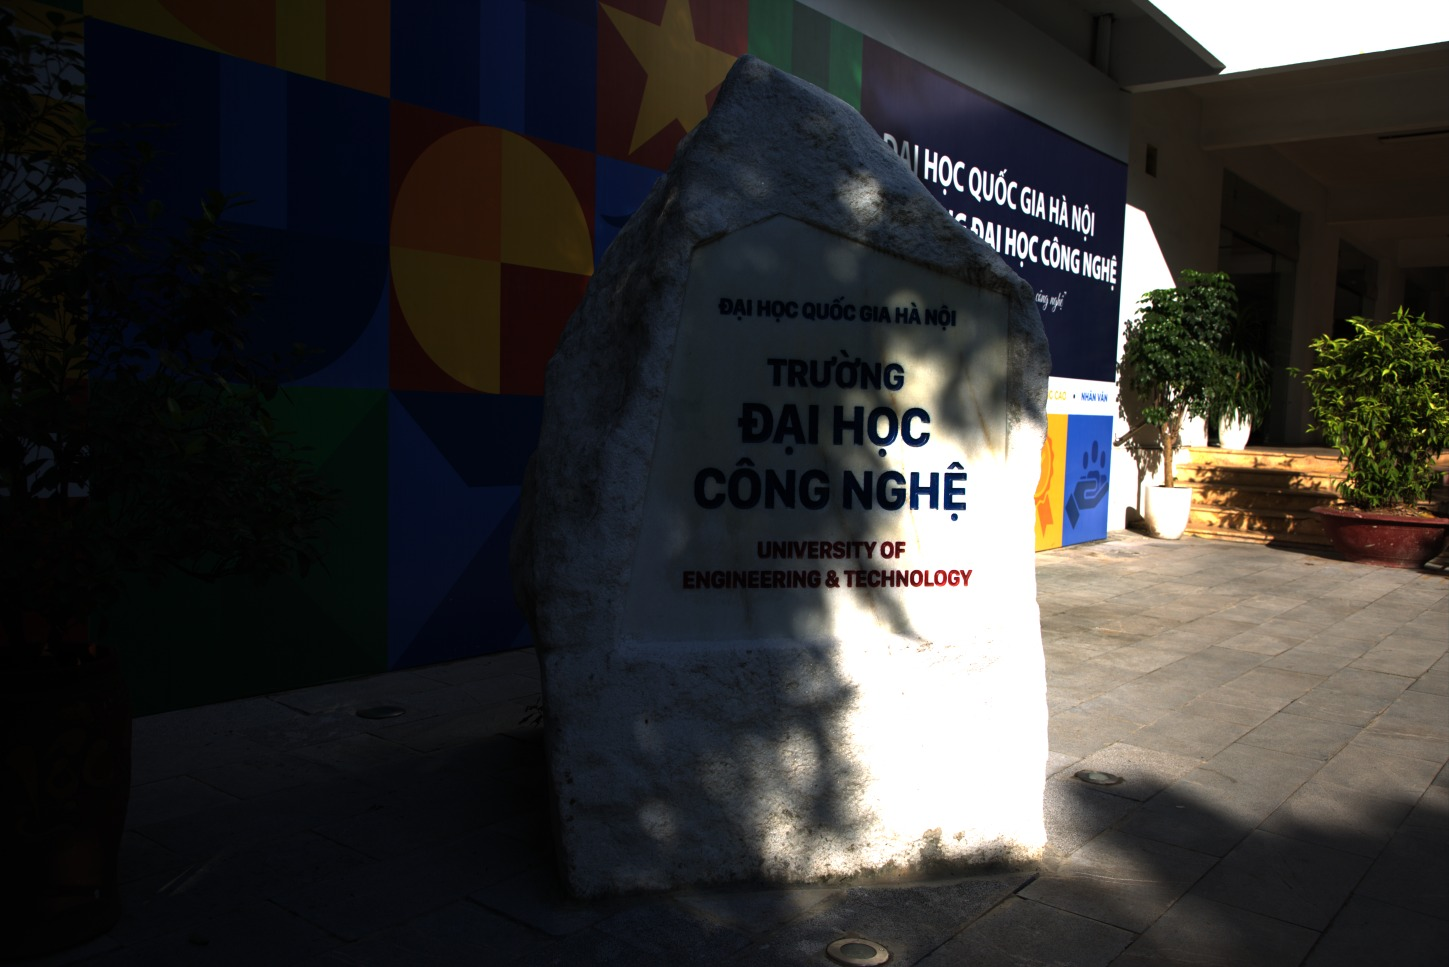
\includegraphics[width=\textwidth]{figures/linear_dark.jpg}
        \caption{Linear, after brightness scaling}
        \label{fig:lin_dark}
    \end{subfigure}
    \hfill
    \begin{subfigure}[b]{0.48\textwidth}
        \centering
        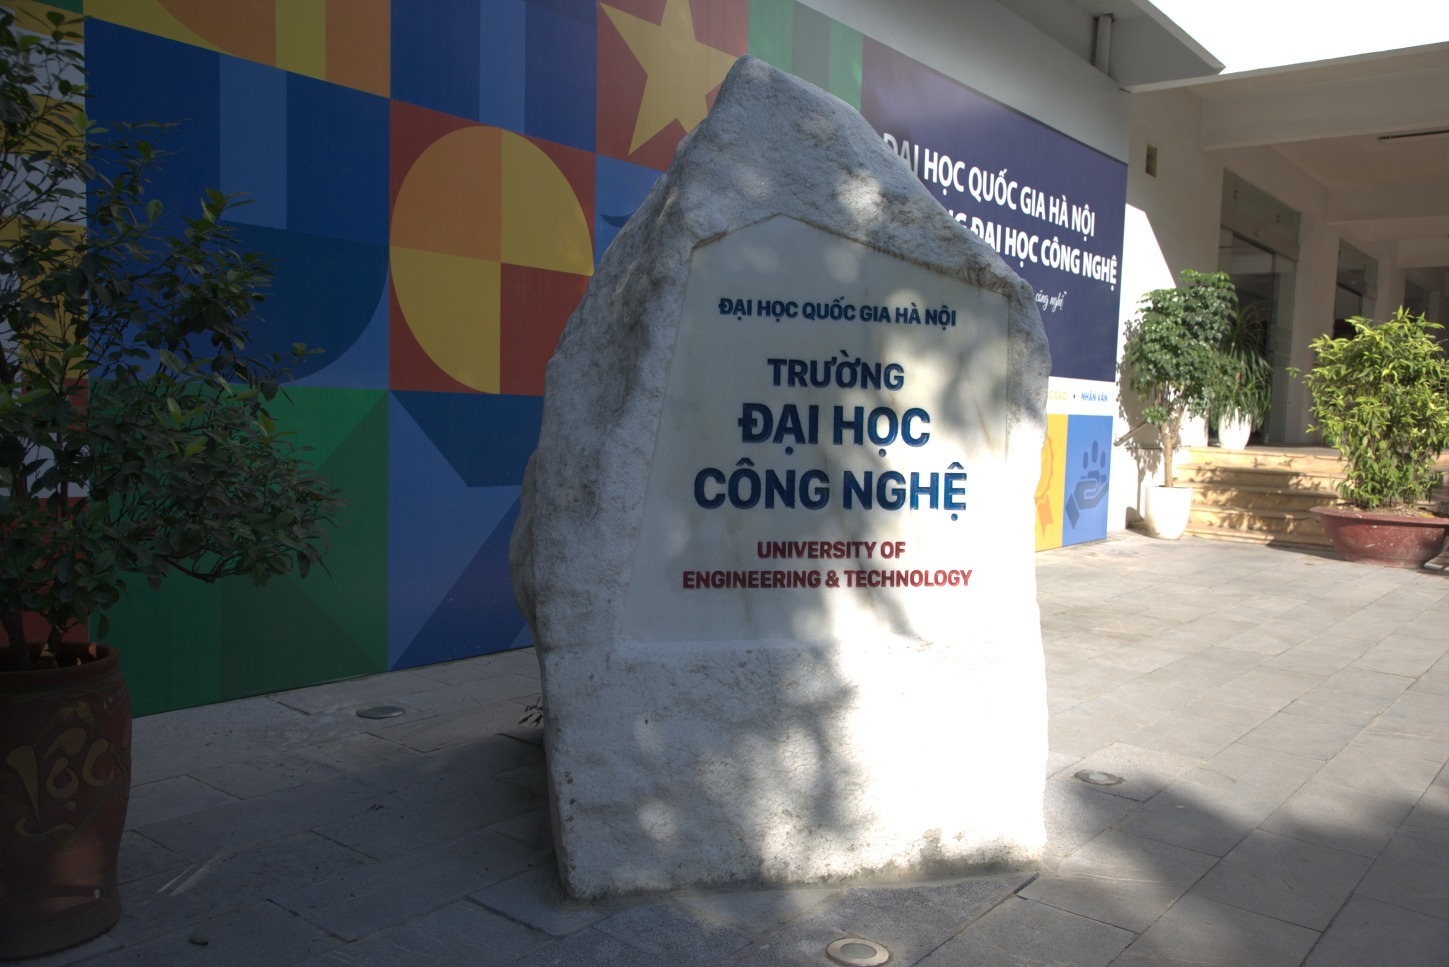
\includegraphics[width=\textwidth]{figures/gamma_encoded.jpg}
        \caption{After sRGB gamma encoding}
        \label{fig:gamma_bright}
    \end{subfigure}
    \caption{Comparison between the linear image and the gamma-encoded image.}
    \label{fig:gamma_comp}
\end{figure}

\section{Compression}

\subsection{Implementation}
The floating-point sRGB image in $[0, 1]$ is converted to 8-bit integers (\texttt{uint8}) with \texttt{img\_as\_ubyte} from \texttt{skimage} and exported as a lossless PNG file and a lossy JPEG file:
\begin{lstlisting}
def save_png_jpeg(self, prefix: str, quality: int = 95):
    img_8bit = img_as_ubyte(np.clip(self.rgb_srgb, 0.0, 1.0))
    png_path, jpg_path = f"{prefix}.png", f"{prefix}.jpg"
    io.imsave(png_path, img_8bit)
    io.imsave(jpg_path, img_8bit, quality=quality)
    png_kb = os.path.getsize(png_path) / 1024.0
    jpg_kb = os.path.getsize(jpg_path) / 1024.0
    ratio = png_kb / jpg_kb
    return png_kb, jpg_kb, ratio
\end{lstlisting}

\subsection{Comparison}
The final image was saved as PNG and as JPEG at six quality settings. Table~\ref{tab2} lists the file sizes and the compression ratio (PNG size divided by JPEG size).

\begin{table}[H]
\centering
\caption{File size and compression ratio at different JPEG qualities compared to PNG}
\label{tab2}
\begin{tabular}{lcc}
\toprule
\textbf{File} & \textbf{File Size (KB)} & \textbf{Compression Ratio} \\
\midrule
PNG (lossless)     & $27710.19$ & $1.00\times$ \\
JPEG, quality 95   & $4311.16$  & $6.43\times$ \\
JPEG, quality 85   & $2034.11$  & $13.62\times$ \\
JPEG, quality 75   & $1416.62$  & $19.56\times$ \\
JPEG, quality 50   & $897.99$   & $30.86\times$ \\
JPEG, quality 25   & $606.93$   & $45.66\times$ \\
JPEG, quality 10   & $433.01$   & $63.99\times$ \\
\bottomrule
\end{tabular}
\end{table}

At the quality required by the assignment ($95$), the JPEG is $6.43\times$ smaller than the PNG ($4.3$~MB instead of $27.7$~MB).

Compression artifacts cannot be seen in a full-frame reproduction, so Figure~\ref{fig:jpeg_crops} shows the same $180 \times 120$ pixel region of every file, enlarged $5\times$ without smoothing. The region contains fine marble texture and saturated red letters on a light background, which is where JPEG fails first.

\begin{figure}[H]
    \centering
    \begin{subfigure}[b]{0.32\textwidth}
        \centering
        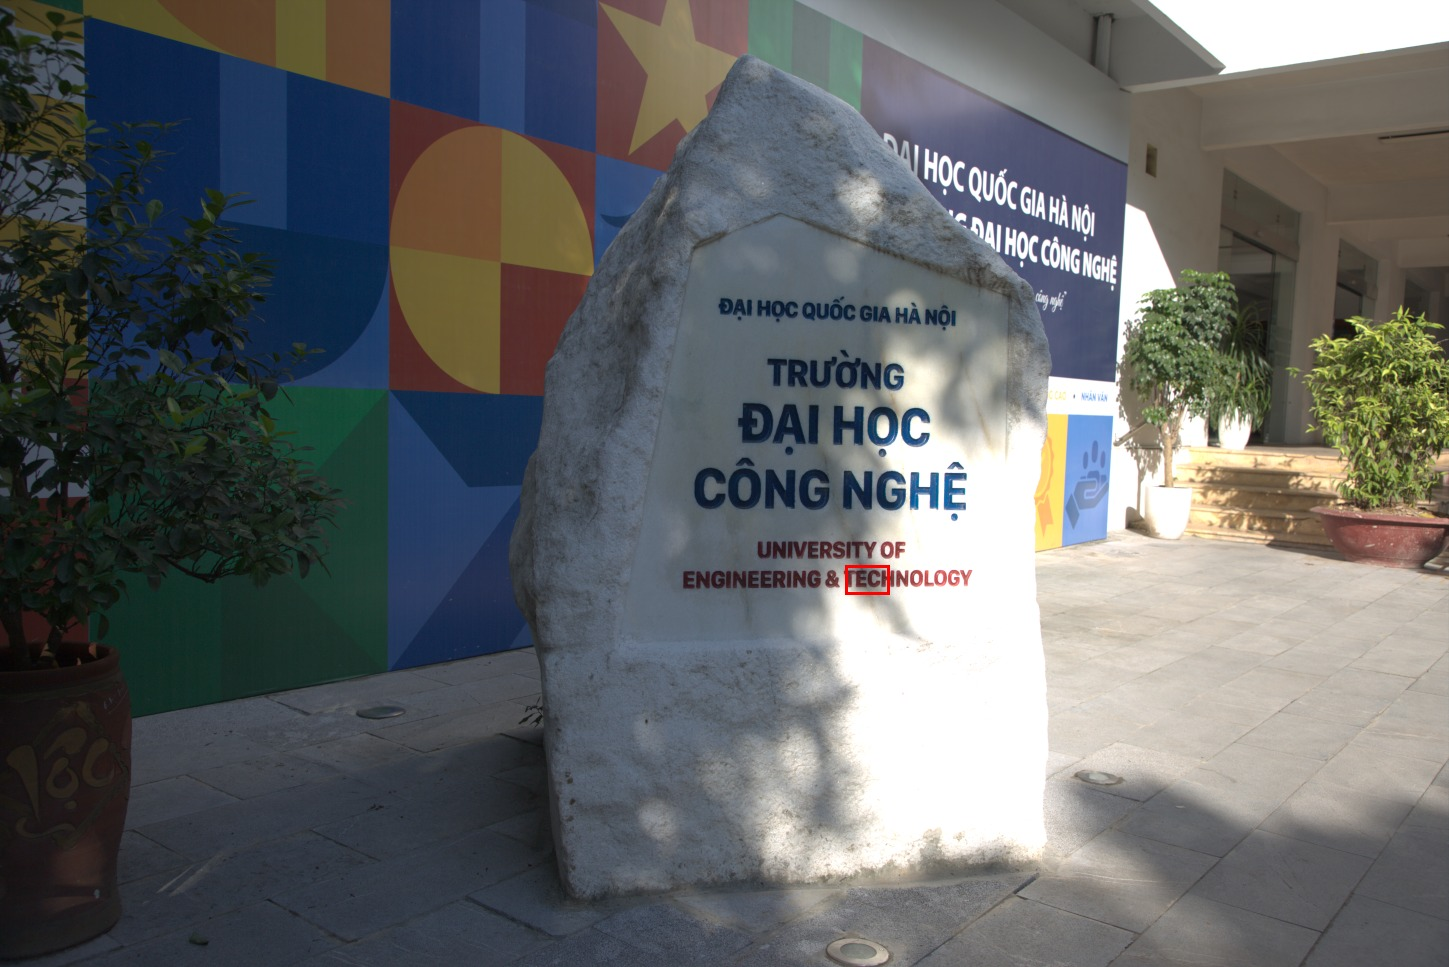
\includegraphics[width=\textwidth]{figures/jpeg_crop_location.jpg}
        \caption{Final image; red frame: region}
    \end{subfigure}
    \hfill
    \begin{subfigure}[b]{0.32\textwidth}
        \centering
        
\includegraphics[width=\textwidth]{figures/jpeg_crop_png.png}
        \caption{PNG, $27710$ KB}
    \end{subfigure}
    \hfill
    \begin{subfigure}[b]{0.32\textwidth}
        \centering
        
\includegraphics[width=\textwidth]{figures/jpeg_crop_q95.png}
        \caption{Quality 95, $4311$ KB}
    \end{subfigure}

    \vspace{0.3cm}
    \begin{subfigure}[b]{0.32\textwidth}
        \centering
        
\includegraphics[width=\textwidth]{figures/jpeg_crop_q85.png}
        \caption{Quality 85, $2034$ KB}
    \end{subfigure}
    \hfill
    \begin{subfigure}[b]{0.32\textwidth}
        \centering
        
\includegraphics[width=\textwidth]{figures/jpeg_crop_q75.png}
        \caption{Quality 75, $1417$ KB}
    \end{subfigure}
    \hfill
    \begin{subfigure}[b]{0.32\textwidth}
        \centering
        
\includegraphics[width=\textwidth]{figures/jpeg_crop_q50.png}
        \caption{Quality 50, $898$ KB}
    \end{subfigure}

    \vspace{0.3cm}
    \begin{subfigure}[b]{0.32\textwidth}
        \centering
        
\includegraphics[width=\textwidth]{figures/jpeg_crop_q25.png}
        \caption{Quality 25, $607$ KB}
    \end{subfigure}
    \hspace{0.02\textwidth}
    \begin{subfigure}[b]{0.32\textwidth}
        \centering
        
\includegraphics[width=\textwidth]{figures/jpeg_crop_q10.png}
        \caption{Quality 10, $433$ KB}
    \end{subfigure}
    \caption{The same region of the PNG and of each JPEG file, with the size of the whole file.}
    \label{fig:jpeg_crops}
\end{figure}

\textbf{Lowest Indistinguishable Quality:} Comparing each JPEG file with the PNG side by side at normal ($100\%$) size, I could not see any difference down to \textbf{quality 50}. Only under the $5\times$ magnification of Figure~\ref{fig:jpeg_crops} does quality $50$ show a slight smoothing of the fine marble grain, which is invisible at normal size. Below this setting the losses become visible: at quality $25$ the $8 \times 8$ blocks and the color smearing around the red letters can be seen without magnification, and at quality $10$ the image is clearly degraded. I therefore take \textbf{quality 50} as the lowest setting that is visually indistinguishable from the PNG. Its file is $897.99$~KB against $27710.19$~KB for the PNG, a compression ratio of $30.86\times$ (a $96.8\%$ reduction).

\section{Statement of AI Usage}
In accordance with the assignment guidelines, I used an AI assistant (Google Gemini) as a supporting tool in the following ways:
\begin{itemize}
    \item \textbf{Understanding the theory:} clarifying concepts behind the pipeline, such as why the Bayer pattern has twice as many green pixels, how the sRGB gamma curve is defined, and how the color space correction matrix is derived.
    \item \textbf{Implementation support:} suggestions and debugging help for the more involved parts of the code, in particular the bilinear interpolation kernels in \texttt{demosaic\_bilinear()}, the row normalization of the color correction matrix, the parsing of the CR2 file in \texttt{detect\_bayer\_pattern\_from\_cr2()}, and the script that produces the figures.
    \item \textbf{Report formatting:} help with the \LaTeX{} layout of tables, figures, code listings and equations.
\end{itemize}
All AI suggestions were checked against the lecture material, the assignment specification and the cited references, and every result in this report was verified by running the code.

\bibliographystyle{IEEEtran}
\bibliography{reference_01}

\end{document}
